% Packages (fold)
\RequirePackage{lmodern}
\documentclass[12pt, oneside, extrafontsizes]{memoir}  % TODO 12pt, twoside

\setstocksize{11in}{8.5in}
\settrimmedsize{11in}{8.5in}{*}
\settrims{0in}{0in}
\setlrmarginsandblock{38mm}{25mm}{*}
\setulmarginsandblock{25mm}{25mm}{*}
\setheadfoot{13pt}{26pt}
\setheaderspaces{*}{13pt}{*}
\checkandfixthelayout
\DoubleSpacing
\setsecnumdepth{subsubsection}
\headstyles{default}
\chapterstyle{ell}
\setsecheadstyle{\scshape\LARGE\raggedright}

\usepackage[colorlinks,bookmarksnumbered,bookmarksdepth=subsubsection,unicode=true]{hyperref}
\newsubfloat{figure}  % must follow hyperref
\hypersetup{
pdfauthor = {Pierre-Luc Bacon},
pdftitle = {On the Bottleneck Concept for Options Discovery: Theoretical Underpinnings and Extension in Continuous State Spaces},
pdfsubject = {Subject},
pdfkeywords = {reinforcement learning, markov chains, hierarchical reinforcement learning},
pdfcreator = {LaTeX with the hyperref package},
pdfproducer = {},
linkcolor = [HTML]{000000},
citecolor = [HTML]{0000FF},
%urlcolor = [HTML]{\colorc}
}
\usepackage{amsmath}
\usepackage{amsfonts}
\usepackage{amssymb}
\usepackage{amsthm}
\usepackage{dsfont}
\usepackage{xspace}
\usepackage{tikz}
\usetikzlibrary{shapes,arrows}
\usepackage{standalone}
\usepackage[boxed]{algorithm2e}

% Custom commands
\newcommand{\rvs}{r.v.'s\xspace}
\newcommand{\mdp}{Markov Decision Process\xspace}
\newcommand{\mdps}{Markov Decision Processes\xspace}
\newcommand{\mrp}{Markov Reward Process\xspace}
\newcommand{\mc}{Markov Chain\xspace}

\def\given{\;\middle\vert\;}
\def\optimal{\star}
\def\transpose{\intercal}
\def\laplacian{\mathbf{\mathcal{L}}}
\def\eqdef{\overset{\underset{\mathrm{def}}{}}{=}}
\def\indicator{\mathds{1}}
\DeclareMathOperator{\expectation}{\mathbb{E}}
\DeclareMathOperator{\vol}{\text{vol}}

\newcommand{\todo}[1]{[TODO: #1]}
\newcommand{\termidx}[1]{\index{#1}{\textbf{#1}}}

\theoremstyle{plain}
\newtheorem{thm}{Theorem}[section]
\newtheorem{lem}[thm]{Lemma}
\newtheorem{prop}[thm]{Proposition}
\newtheorem*{cor}{Corollary}

\theoremstyle{definition}
\newtheorem{defn}{Definition}[section]
\newtheorem{conj}{Conjecture}[section]
\newtheorem{exmp}{Example}[section]

\usepackage[utf8]{inputenc}
\usepackage{csquotes}
\usepackage{showidx}
\makeindex

\usepackage[backend=biber, citestyle=authoryear, bibstyle=authoryear, isbn=false, url=false, doi=false, eprint=false, natbib=false, sorting=nty, uniquename=init]{biblatex}
\addbibresource{library.bib}

\begin{document}

%%%%%%%%%%%%%%%%%%%%%%%%%%%%%%%%%%%%%%%%%%%%%%%%%%%%%
% Title page
%%%%%%%%%%%%%%%%%%%%%%%%%%%%%%%%%%%%%%%%%%%%%%%%%%%%%

% Title (fold)
\pretitle{\begin{center}\cftchapterfont\huge}
\posttitle{\end{center}}
\preauthor{\begin{center}\huge}
\postauthor{\end{center}}
\predate{\begin{center}\large}
\postdate{\end{center}}

\title{On the Bottleneck Concept for Options Discovery: \\ \large{Theoretical Underpinnings and Extension in Continuous State Spaces} }
\author{Pierre-Luc Bacon}
\date{\today}
\renewcommand\maketitlehookb{
\vfill
}
\renewcommand\maketitlehookc{
\vfill
\begin{center}
{
\large
Computer Science\\
McGill University, Montreal
}
\end{center}
\vspace{10mm}
}
\renewcommand\maketitlehookd{
\vspace{10mm}
A thesis submitted to McGill University in partial fulfilment of the requirements of
the degree of Master of Science.
\copyright Pierre-Luc Bacon; \today.
}
% Title (end)

\begin{titlingpage}
\maketitle
\end{titlingpage}

%%%%%%%%%%%%%%%%%%%%%%%%%%%%%%%%%%%%%%%%%%%%%%%%%%%%%
% Ackowledgements
%%%%%%%%%%%%%%%%%%%%%%%%%%%%%%%%%%%%%%%%%%%%%%%%%%%%%
%\clearpage
%\pagenumbering{roman}
%\renewcommand{\abstractname}{Dedication}

%%%%%%%%%%%%%%%%%%%%%%%%%%%%%%%%%%%%%%%%%%%%%%%%%%%%%
% Ackowledgements
%%%%%%%%%%%%%%%%%%%%%%%%%%%%%%%%%%%%%%%%%%%%%%%%%%%%%
\clearpage
\pagenumbering{roman}
\renewcommand{\abstractname}{Acknowledgements}
\begin{abstract}
I would like to thank everyone with whom I had the chance to share my 
enthusiasm upon exploring new ideas; those who gave me the freedom to fail, thinker,
and be slightly obsessed on certain days.

I am deeply grateful to my supervisor Doina Precup, Amir-massoud Farahmand, and Gheorghe Comanici for their precious insights and encouragement. Special thanks to lab members Clement Gehring and Neil Girdhar for their persistence in constructively challenging my ideas.
\end{abstract}

%%%%%%%%%%%%%%%%%%%%%%%%%%%%%%%%%%%%%%%%%%%%%%%%%%%%%
% Abstract
%%%%%%%%%%%%%%%%%%%%%%%%%%%%%%%%%%%%%%%%%%%%%%%%%%%%%
\clearpage
\renewcommand{\abstractname}{Abstract}
\begin{abstract}
The bottleneck concept in reinforcement learning has played a prominent role in automatically finding temporal abstractions from experience. Lacking significant theory, it  has however been regarded by some as being merely a \textit{trick}. This thesis attempts to provide elements from spectral graph theory to support it while also gaining better intuition about its shortcomings. A connection to the theory of Nearly Decomposable Markov Chains is also drawn and shows great promise. An options discovery algorithm explainable in terms of spectral graph clustering is proposed and is the first of its kind to be applicable in continuous state spaces. As opposed to other similar approaches, this one has running time $\mathcal{O}(mn^2)$ rather than $\mathcal{O}(n^3)$ making it suitable to much larger domains than the typical \textit{grid worlds}.
\end{abstract}

%%%%%%%%%%%%%%%%%%%%%%%%%%%%%%%%%%%%%%%%%%%%%%%%%%%%%
% Abrégé
%%%%%%%%%%%%%%%%%%%%%%%%%%%%%%%%%%%%%%%%%%%%%%%%%%%%%
\clearpage
\renewcommand{\abstractname}{Résumé}
\begin{abstract}
L'identification automatique de goulots d'étranglement dans la structure de solution a joué un rôle important en apprentissage par renforcement hiérarchique au cours des dernières années. Bien que populaire, cette approche manque toujours de fondements théoriques adaptés. Ce mémoire tente de pallier ces lacunes en établissant des liens en théorie spectrale des graphes, espérant ainsi obtenir une meilleure compréhension des conditions garantissant son applicabilité. Une revue des efforts réalisés concernant les chaines de Markov presque complètement décomposable (NCD) permet de croire qu'elles pourraient être utiles au problème ici considéré. Un algorithme de découverte d'options motivé par la théorie spectrale des graphes est proposé et semble être le premier du genre à pouvoir être aussi appliqué dans un espace d'états continu. Contrairement à d'autres approches similaires, la complexité algorithmique en temps est de l'ordre de $\mathcal{O}(mn^2)$ plutôt que $\mathcal{O}(n^3)$, rendant possible la résolution de problèmes de plus grande envergure.
\end{abstract}

%%%%%%%%%%%%%%%%%%%%%%%%%%%%%%%%%%%%%%%%%%%%%%%%%%%%%
% Table of content
%%%%%%%%%%%%%%%%%%%%%%%%%%%%%%%%%%%%%%%%%%%%%%%%%%%%%
\clearpage
\setcounter{tocdepth}{2}
\tableofcontents
%\newpage
%\listoffigures
%\listofalgorithms

%%%%%%%%%%%%%%%%%%%%%%%%%%%%%%%%%%%%%%%%%%%%%%%%%%%%%
% Introduction
%%%%%%%%%%%%%%%%%%%%%%%%%%%%%%%%%%%%%%%%%%%%%%%%%%%%%
\clearpage
\pagenumbering{arabic}
\chapter{Introduction}
With the breakthroughs in hierarchical reinforcement learning (HRL) at the beginning of the last
decade, temporal abstraction has been expected to play an central role in scaling up currently
known techniques to new levels. Its development however still seems to be hindered by an
easily explainable, yet challenging problem: how can temporal abstractions be discovered
automatically ? This is the "elephant in the room" for HRL. The existence of this problem has
been acknowledged by many authors who also called for the need to develop efficient
techniques to adress it. The author of the MAXQ framework even went to qualify it as being the
"biggest open problem" \cite{Dietterich2000} in HRL. Without automatic methods for
decomposing the problem structure into simpler sub-problems, hierarchical approaches are of
limited interest as the effort for manually specifying them can quickly become insurmountable. 
In one attempt to jointly solve state and temporal abstraction, the author of the HEXQ algorithm
goes on to refer to manual task decomposition as a quasi ``art-form'' \cite{Hengst2002}.

The bottleneck concept arose early in the field of HRL as an intuitive response to this issue. Bottlenecks have been defined as those states which appear frequently on successful trajectories to a goal but not on unsuccessful ones~\cite{Mcgovern2001, Stolle2002} or as nodes which allow for densely connected regions of the interaction graph to reach other such regions~\cite{Menache2002, Simsek2004, Kazemitabar2009}. \cite{Simsek2004} qualifies such states as \textit{access states}, allowing difficult regions of the state space to be reached. The canonical example of bottleneck states often refers to \textit{doorways} in a navigation problem across rooms of a grid-world domain.

\section{Graph Clustering Perspective}
The ideas presented in this thesis found their roots early in the history or HRL. It
will be argued in chapter \ref{chap:dynamics}  that bottlenecks are intrinsically related to graph
clustering. \cite{Hauskrecht1998} had already envisioned such a state-space partitioning
approach leading to an abstract MDP being overlaid to the \textit{periphery} of the partitions.
\textit{Macro-actions} would then be learnt to transition between such abstract peripheral
states. While it is assumed that such a decomposition is provided, it is shown that such a model
can lead to a reduction in the size of the state or action spaces. A similar state-space
partitioning intuition had also been explored in \cite{Dean1995} by one of the co-author of the
previous paper. While the method of \cite{Dean1995} was not cast yet under the framework of
reinforcement learning, it showed how a global planning problem could be decomposed into
smaller locally-solvable problems which could be then be recombined into an optimal policy.
The machinery or HRL being in its infancy, Dantzig-Wolfe method \cite{Dantzig1960} of
decomposition (a linear programming algorithm) was used to solve the abstract MDP. The
problem of obtaining a proper partitioning is also sidestepped in this work.

Along the same line of work, \cite{Menache2002} also proposed a decomposition algorithm called \textsc{Q-Cut} based on graph partitioning view of the state transition graph. The Max-Flow/Min-Cut algorithm is used for finding the bottleneck states and flat policies are constructed to reach them. The problem of learning the policy over the problem decomposition is then cast under the options framework \cite{Sutton1999} where the \textsc{SMDP Q-Learning} algorithm is applied. The approach is revisited in \cite{Mannor2004} where an agglomerative graph clustering is applied. Under this slightly modified perspective, temporal abstraction takes place between pairs of clusters rather than from arbitrary states to bottleneck states. Two type of clusterings are also differentiated: \textit{topological} and \textit{value-based}. The former attempts to group states into clusters based on structural regularities of the environment while the latter considers the reward information collected during learning.
This agglomerative approach has recently been reformulated under an online setting in the \textit{Online Graph-based Agglomerative Hiearchical Clustering} algorithm (\textsc{OGAHC}) of \cite{Metzen2012}.

The \textsc{L-Cut} algorithm of \cite{Simsek2005} can be seen as an extension of \textsc{Q-Cut} subject to the constraint of a local knowledge of the environment. Rather than setting up the graph bisection problem under the Max-Flow/Min-Cut formulation, the \textsc{NCut} criterion of \cite{ShiMalik2000} is used to measure the quality of the partitioning and is solved as as generalized eigenvalue problem. A local graph representation is obtained by collecting samples of experience through a random walk process. After a certain number of iterations, the spectral bipartionning algorithm is applied and a policy, encoded as an \textit{option}, is learnt to reach the identified subgoals. A statistical test is applied on the set of boundary states of each partition to discriminate \textit{useful} subgoals from noise.

The spectral clustering approach was revisited more recently in \cite{Mathew2012} under the Robust Perron Cluster Analysis of \cite{Weber2004} and its \textsc{PCCA+} algorithm. While \textsc{NCut} and \textsc{PCCA+} are both spectral techniques sharing much in common,  Perron Cluster Analysis lends itself more easily to an interpretation in terms of metastability and invariant subsets of a Markov chain. Intuitively, metastable regions corresponds to subsets of states in which the stochastic process spends more time, switching to other such subsets on rare occasions. The \textit{cascade decomposition} technique of \cite{Chiu2010} attempts to find bottlenecks by computing the second eigenvector of the normalized graph Laplacian. It is in essence very similar to \textsc{L-Cut} which uses \textsc{NCut} \cite{ShiMalik200}, also derived from the normalized graph Laplacian. 

Trying to address both the discovery problem and the related one of transfer learning, \cite{Bouvrie2012} builds upon the diffusion maps framework of \cite{Coifman2006} and sharing ideas from \cite{Mahadevan2007}. A spectral partitioning approach is also taken to identify \textit{geometric bottlenecks} of the environment without taking the reward structure into consideration. The diffusion framework is defined in terms of the random walk process on a graph and the spectrum of the corresponding normalized graph Laplacian \cite{Chung1997}. The uniqueness of this other instance of the graph partitioning approach to temporal abstraction lies its ability to \textit{blend} policies and reward functions found at different levels of abstraction. 

Rather than searching for a general partitioning of the state space, \cite{Kazemitabar2009} attempts to find strongly connected components (SCC). While similar in spirit, the idea of finding such structures raise some questions regarding ergodic properties. It seems indeed that this scheme could be highly sensible to the sampling strategy. It could be expected that in most situations, only a single component would be found. In short, the SCC constraint seems to be too strong. Surprisingly, the \textsc{HEXQ} framework of \cite{Hengst2002} is not mentioned by  the authors. \textsc{HEXQ} also attempts to automatically discover hierarchical structure based on the analysis of the SCC decomposition of each state variable. The author gives an interpretation of the resulting decomposition in terms of maximum \textit{predictability} within those regions. Such a view also admits an information theoretic interpretation which is hinted to the reader later in this thesis.

\section{States Classification Approaches}
Rather than explicitly partitioning the state space using graph theoretic tools, another body of work focused on directly classifying out bottleneck states based on a visitation frequency principle. This view of bottleneck detection is in a sense more aligned with the philosophical principle of reinforcement learning. Indeed, it tends to lend itself more easily to an online formulation and is cheap to compute. The proposed solutions are however deeply heuristic-based and it quickly becomes difficult to determine which of them might be superior. While little theory is also known about the class of graph partitioning approaches, it seems easier to back it up with meaningful theory as argued in chapter \ref{chap:dynamics}.

The bottleneck discovery problem is formulated in \cite{Mcgovern2001} as a multiple-instance learning problem over bags of feature vectors collected by interacting with the environment. Two sets of bags are obtained in this way: from observations collected along successful and unsuccessful trajectories respectively. The notion of diverse density is then applied  either by exhaustive search or gradient descent to find regions of the feature space with the most positive instances and the least negative ones. Because negative bags must only contain unsuccessful trajectories, while positive bags have to contain at least one successful feature vector, this method is sensitive to noise. The classification constraint imposed  by \cite{Mcgovern2001} between \textit{good} and \textit{bad} trajectories is lifted in \cite{Stolle2002}. It rather directly extracts those states which have been visited frequently and define them as subgoals. The initiation sets of the options is found by interpolating between over the states which appear frequently enough (above average) on the paths going through those maxima.

In~\cite{Simsek2004}, the authors identify subgoals by looking for \textit{access states} which lead to the regions of the state space that have not been visited recently and trying to capture the notion of \textit{relative novelty}. The time frame within which to search for such novelty events is a parameter of this algorithm and influences the results obtained.

The use of a standard network centrality measure called \textit{betweenness centrality} is investigated in \cite{Simsek2008}. Betweenness centrality measures the fraction of shortest paths passing through a given vertex of the graph. Nodes with high betweenness are deemed more important as they would appear more frequently on trajectories to the goal. The reward function is somehow taken into account into this measure by weighting the paths depending on weather they successfully reached the goal or not. A new graph centrality measure is proposed in \cite{Rad2010} called \textit{connection graph stability} and is argued empirically to be a better fit than betweenness centrality for discovering bottlenecks. The same group of authors then exploited slight variations of this definitions under different names such as \textit{connection bridge centrality} or \textit{co-betweenness centrality} \cite{Moradi2010}.  

compute betweenness centrality to identify important subgoals. They
also propose a potential incremental formulation of their algorithm
that finds local maxima of betweenness within the subgraph obtained
by collecting short trajectories. However, it has also been argued~\cite{Rad2010} that
the centrality measure called \textit{connection graph stability} leads
to better subgoal identification than betweenness or closeness centrality.

\subsection{Outline}

Basic theory of stochastic processes and Markov chains is first presented in chapter \ref{chap:decisionmaking}. The inclusion of this material is motivated by the probabilistic interpretation of spectral graph theory studied in chapter \ref{chap:dynamics}. The theory of Markov Decision Processes is presented in section \ref{sec:mdp} as a necessary prerequisite to the appreciation of the techniques developed in reinforcement learning. Chapter \ref{chap:temporalabstraction} focuses on the presentation of the options framework \cite{Sutton1999} in reinforcement learning as a way to express temporal abstraction and learn optimal policies over such hierarchical representation. 

The connection from graph \textit{structure} to system \textit{dynamics} is developed throughout chapter \ref{chap:dynamics} and is instrumental is understanding the strengths and pitfalls of the graph partitioning approach to options discovery. It also allows a better understanding of the relevance of the work on Nearly-Completely Decomposable Markov Chains (NCD) towards better theoretical developments on the bottleneck concept. Furthermore, the perturbational approach traditionally taken in this field hints to an information theoretic comprehension of temporal abstraction. 

A new algorithm for options discovery is developed in chapter \ref{chap:buildingoptions} based on the community detection algorithm \textsc{Walktrap} of \cite{Pons2005}. Although \textsc{Walktrap} finds its roots into spectral graph theory, its running time is order $\mathcal{O}(mn^2)$ rather than $\mathcal{O}(n^3)$ by avoiding to compute the eigenvectors explicitly. The problem of options discovery and construction is also set under the assumption of a continuous space. Techniques for constructing proximity graphs are also developed in section \ref{sec:proximitygraphs}. It is also shown how approximate nearest neighbors algorithms can be used to properly define the initiation and termination components of the options when subject to continuous observations.

An illustration of the proposed algorithm is provided in chapter \ref{chap:illustration} under the Pinball domain of \cite{Konidaris2009}. Practical difficulties having to do oscillations and off-policy learning are analysed. The proper empirical choices for the number of nearest neighbors, type of proximity graph and time scale for the \textsc{Walktrap} algorithm are discussed.

%%%%%%%%%%%%%%%%%%%%%%%%%%%%%%%%%%%%%%%%%%%%%%%%%%%%%
% Background
%%%%%%%%%%%%%%%%%%%%%%%%%%%%%%%%%%%%%%%%%%%%%%%%%%%%%
\chapter{Sequential Decision Making under Uncertainty}
\label{chap:decisionmaking}
\section{Markov Chains}

A discrete-time stochastic process is a family of random variables $\{ X(t), t \in T\}$
(\rvs) indexed by a time parameter $t \in \mathbb{N} = \{0, 1, 2,...\}$. The
value of $X_n$ is referred to as the \termidx{state} of the process. When the family of
random variables is defined over a discrete sample space
$\Omega$, the stochastic process is said to be \textit{discrete-valued}.
Stochastic processes are useful for modelling probabilistic phenomenon involving in
time such as the evolution of the price of a stock, or the
number of connections to a web service over the day for example. Due to the inherent
complexity many systems, it is often desirable to make simplifying assumptions to
make the exercise tractable. One might then decide to treat the \rvs as
\textit{independent and identically distributed} (iid) but only at the cost of loosing the ability to
capture the correlation structure among the \rvs. The so-called \textit{Markov}
assumption is often used when the iid property is deemed too restrictive, but is yet
simple enough to make computation tractable.

\begin{defn}
A \termidx{Markov Chain} is a discrete-time and discrete-valued stochastic process
which possesses the Markov property. The Markov property implies that for all times $n \geq
0$ and all states $i_0, \dots, i, j \in \Omega$:
\begin{equation}
P(X_{n+1} = j | X_0 = i_0, X_1 = i_1, ..., X_n = i) = P( X_{n+1} = j | X_n = i)
\end{equation}
\end{defn}

The Markov property (or \termidx{memoryless property}) could be stated simply by
saying that the \textit{future is independent of the past, given the present state}.
Therefore, knowing the current value of $X_n = i$ is enough to characterize the
future evolution of the stochastic process $\{X_{n+1}, X_{n+2}, \dots \}$ and the history
$\{X_0, X_1,\dots, X_{n-1} \}$ can be discarded.

A Markov chain is completely specified by the one-step transition probabilities
$p_{ij} = P(X_{n+1} = i | X_n = j)$ contained in its Markov or
\termidx{stochastic matrix}. For a finite state-space $\mathcal{X}$, we have:
\begin{equation}
\mathbf{P} = \begin{bmatrix}
p_{11} & p_{12} & \cdots & p_{1m} \\
p_{21} & p_{22} & \cdots & p_{2m} \\
\vdots & \vdots & \ddots & \vdots \\
p_{m1} & p_{m2} & \cdots & p_{mm}
\end{bmatrix}
\end{equation}

Furthermore, $\mathbf{P} $ must satisfy the following properties:
\begin{equation}
p_{ij} \geq 0 \mbox{ and } \sum_{j=1}^M p_{ij} =1 
\end{equation}

Let $\mathbf{P}^\optimal$ denote the adjoint of $\mathbf{P}$. If $\mathbf{P}^\optimal = \mathbf{P}$ holds, then the stochastic matrix is said to be \termidx{time-reversible}. 

Those elements of $\mathbf{P}$ for which $p_{ii} = 1$ are said to be
\termidx{absorbing} and once entered, the Markov chain the never escapes.

If the elements of $\mathbf{P} $ are independent of the time index, the
Markov chain is said to be \termidx{time-homogeneous} and has \termidx{stationary transition
probabilities}. If this property is satisfied and one knows the transition probabilities of
a Markov Chain, the problem of computing probability distributions is greatly
simplified and can be succinctly expressed using matrix multiplication.  

The \termidx{Chapman-Kolmogorov} equation lets us express the probability of
going from state $i$ to $j$ in $n$ steps by $[\mathbf{P}^n]_{ij} = [
\underbrace{\mathbf{P} \times \mathbf{P} \times \dots \times \mathbf{P}}_{\text{n
times}} ]_{ij}$. The probability of transitioning from state $i$ to any other state under
$n$ steps then becomes:
\begin{equation}
P( \cdot, n | i) = e_i \mathbf{P}^n
\end{equation}
Here $e_i$ stands for the vector with zero components everywhere except of for its
$i$th component set to 1. 

Using the Chapman-Kolmogorov equation, a state $j$ is classified as being
\termidx{accessible} from $i$ if $[\mathbf{P}^n]_{i,j} > 0$ for some $n \geq 0$. When
the relation holds in both direction, $i$ and $j$ are said to \termidx{communicate}. If
every possible pair of states can communicate, the Markov chain is classified as being
\termidx{irreducible}. Given that a state $j$ has been initially encountered once, we
say that it is \termidx{recurrent} if the probability of visiting it again is nonzero. That
is, denote $T_j$ the time at which the chain returns to $j$, the recurrence property
expresses the fact that $P(T_j < \infty | X_0 = j) > 0$. When $E(T_j | X_0) < \infty$,
state $j$ is said to be \termidx{positive recurrent}.

These last definitions are essential for defining the \termidx{ergodicity}
property which is a condition often assumed in the analysis of Markov Decision Processes which will be covered below. 

\begin{defn}
A Markov chain is ergodic if it is irreducible and positive recurrent.
\end{defn}

It occurs often that one is interested in knowing how a given probability distribution
for $X_n$ would evolve in time.  Denote the
distribution of $X_n$ by the row vector $\mu_n$ and the \termidx{initial distribution}
by $\mu_0$. It can seen that the following relation hold
\begin{equation}
 \mathbf{\mu}_n= \mathbf{\mu}_0 \mathbf{P}^n \label{eq:initial-dist}
\end{equation}
by noting that the Markov property implies that
\begin{align}
P(X_0 &= i_0, X_1 = i_1, X_2 = i_2, \dots, X_n = i_n) = \notag \\
&P(X_0 = i_0) P(X_1 = i_1 | X_0 = i_0) P(X_2 = i_2 | X_1 = i_1) \dots P(X_n = i_n |
X_{n-1} = i_{n-1})
\end{align}
and that our Markov chain is time-homogeneous ($\mathbf{P}$ is fixed).

If it happens that the distribution of $\mu_n$ does not change with $n$, then 
 the Markov chain is said to be \termidx{stationary}. 

\begin{defn}
A Markov chain said to be stationary if it satisfies $P(X_0 = i_0, X_1 = i_1, \dots, X_n
= i_n) = P(X_m = i_0, X_{m+1}, \dots, X_{m+n})$ for any $m \in \mathbb{Z_+}$.
\end{defn}

Using \ref{eq:initial-dist}, the stationarity problem for a Markov Chain amounts to
finding a vector $\pi$ such that
\begin{equation}
\mathbf{\pi}^\transpose P = \mathbf{\pi}^\transpose
\end{equation}

The stationary distribution $\mathbf{\pi}^\intercal$ can thus be seen as the left
eigenvector of $\mathbf{P}$ associated with the eigenvalue 1. Furthermore, it must be
that $\sum_k \mathbf{\pi}_k = 1$ in order for $\pi$ to be a well-defined probability
distribution. When the Markov chain reaches the stationary distribution, it is said to be
in its \termidx{steady-state} mode.

An important characterization of the properties of stochastic matrices comes from the
theory of nonnegative matrices in the form of the Perron-Frobenius theorem. First, the spectral radius of a square matrix is defined as 

\begin{equation}
\rho(A) \overset{\underset{\mathrm{def}}{}}{=} \max_i(|\lambda_i|)
\end{equation}

The theorem in its original form about irreducible matrices \cite{Horn1986} then amounts to the following.

\begin{thm}[Perron-Frobenius Theorem]

Let $A$ be an irreducible and nonnegative matrix, then the following claims hold
\begin{enumerate}
\item The spectral radius $\rho(\mathbf{A})  > 0$
\item $\rho(\mathbf{A})$ is an eigenvalue of $\mathbf{A}$
\item There exists a positive vector $\mathbf{x}$ such that $\mathbf{A}\mathbf{x} = \rho(\mathbf{A})\mathbf{x}$ and $\rho(\mathbf{A})$ is a simple eigenvalue of $\mathbf{A}$.
\item The unique eigenvector whose components sum to 1 is called \termidx{Perron
 vector}, that is
\begin{equation}
\mathbf{A} \mathbf{p} = \rho(\mathbf{A}) \mathbf{p}, \hspace{2.5mm} \mathbf{p} > 0 \hspace{2.5mm} \mbox{and} \hspace{2.5mm} \|\mathbf{p}\|_1 = 1
\end{equation}
\end{enumerate}
\end{thm}

The theorem can also be conveniently adapted to Markov chains under the following
lemma proven in \cite{Montenegro2006}.
\begin{lem}
Let $\mathbf{P}$ be the stochastic matrix associated with a irreducible and reversible 
Markov chain over a state space $\mathcal{X}$ of size $n$. $\mathbf{P}$ must then
have a complete spectrum of real eigenvalues of magnitude at most 1 and of the form
\begin{equation}
1 = \lambda_0 \geq \lambda_1 \lambda \geq \dots \geq \lambda_{n-1} \geq -1
\end{equation}
\end{lem}

%%%%%%%%%%%%%%%%%%%%%%%%%%%%%%%%%%%%%%%%%%%%%%%%%%%%%
% Markov Decision Processes
%%%%%%%%%%%%%%%%%%%%%%%%%%%%%%%%%%%%%%%%%%%%%%%%%%%%%
\section{Markov Decision Processes}
\label{sec:mdp}
Markov chains of the kind presented in the last section do not consider the influence of an external \textit{input} on its dynamics. The case of controlled Markov chains under the framework of \mdps is studied in this section. The theory of \mdps will lay the theoretical foundations for the problem of optimal sequential decision making for situated agents considered in Reinforcement Learning. The following presentation adopts most of the notion from \cite{Csaba2010}. 

\begin{defn}
\label{defn:mdp}
A finite-action discounted \termidx{Markov Decision Process} (MDP) is a tuple
$\mathcal{M} = \langle \mathcal{X}, \mathcal{A}, r, \mathcal{P},\gamma \rangle$ where
$\mathcal{X}$ is a non-empty countable set of states, $\mathcal{A}$ is a finite state
of actions, $\mathcal{P}$ is a transition probability kernel giving rise to a distribution
$P(\cdot |x, a)$ over $\mathcal{X}$ given any $x \in \mathcal{X}$ and $a \in
\mathcal{A}$,  $r$ is the reward function $r: \mathcal{X} \times \mathcal{A} \mapsto
\mathbb{N}$ and $\gamma \in [0, 1]$ is a discount factor.
\end{defn}

A \termidx{deterministic policy} $\pi$ is a mapping $\pi : \mathcal{X} \mapsto
\mathcal{A}$. In the theory of MDPs, stochastic policies of the form $\pi : \mathcal{X}
\mapsto \Omega(\mathcal{A})$ are also object of study, in which case actions are
drawn from a conditional probability distribution  over states according to $A_t \sim
\pi(\cdot | X_t)$ (here $A_t$ and $X_t$ denote \rvs at time $t$). 

Fixing a policy for an MDP has for effect to induce a \termidx{Markov Reward Process}
(MRP) $\langle \mathcal{X}, \mathcal{R}^\pi, \mathcal{P}^\pi, \gamma \rangle$ with
the reward function $\mathcal{R}^\pi(x) = r(x, \pi(x))$ and state transition probability
kernel $P(\cdot | x) = P(\cdot | x, \pi(x))$. An MRP can be thought as a Markov chain
augmented with rewards over the set of states. The concepts of induced Markov
chains and Markov Reward Processes are particularly important in the analysis of the
dynamics of an MDP. At the level of the induced Markov chain of an MDP, the
existence of a stationary distribution is not necessarily guaranteed.

\subsection{Value Function}
The notion of a value function is instrumental in supporting the principle of optimality
that underlies the decision theoretic framework of MDPs. It is assumed in this context
that a decision maker, or \textit{agent}, is acting in such a way as to optimize some
intrinsic notion of what \textit{good} behaviour is. From to the definition
\ref{defn:mdp} of an MDP, the reward function $r$ is used to express a quantity
known as the \termidx{return}

\begin{defn}
The return of an \mdp is the total discounted sum of the rewards originating from
the induced \mrp.
\begin{equation}
\mathcal{R} = \sum_{t=0}^\infty \gamma^t R_{t+1} \label{eq:return}
\end{equation}
\end{defn}

Fixing the value of $\gamma < 1$ leads to a notion of return where the immediate
reward is worth exponentially more than the far future. In this case, the resulting MDP 
is then called a \termidx{discounted \mdp}. On the other hand, setting $\gamma =
1$ makes the immediate reward observed at each step equally important and one 
then talks of an \termidx{undiscounted \mdp}

Knowing the \textit{desirability}, or value, of a state at any moment will greatly
simplify the problem of deriving an optimal behavior. 

\begin{defn}
The \termidx{value function} $V^\pi: \mathcal{X} \mapsto \mathbb{R}$ of a
stationary policy $\pi$ is the conditional expectation of the return (discounted or
undiscounted) given a state.
\begin{equation} 
V^\pi(x) = \expectation \left[ \sum_{t=0}^\infty \gamma^t R_{t+1}  \given  X_0 =
x\right] , x \in \mathcal{X} \label{eq:value-function}
\end{equation}
\end{defn}

An optimal behavior is achieved if the value function of its policy is optimal. An
optimal value function $V^*: \mathcal{X} \mapsto \mathbb{R}$ is one which obtains
the maximum possible expected return for every state.

% Action value function 
The \termidx{action-value function} of a policy $\pi$ is tightly related to the notion of
value function presented above. Instead of being defined only over states, it specifies
the expected return of initially being in state $x$ choosing a first action $a$ and
following $\pi$. 
\begin{defn}
The action-value function $Q^\pi: \mathcal{X} \times \mathcal{A} \mapsto
\mathbb{R}$ of a stationary policy $\pi$ is the conditional expectation of the return
given an initial state and action pair. 
\begin{equation}
Q^\pi(x, a) = \expectation \left[ \sum_{t=0}^\infty \gamma^t R_{t+1} \vert X_0 = x,
A_0 = a \right], \; x \in \mathcal{X}, a \in \mathcal{A}
\end{equation}
\end{defn}

If the action-value function yields the maximum expected return for every state
action pair, it is said to be optimal and denote it by $Q^*$. One can go from the
action-value function to the value-function by noting that for finite-action MDP
(definition \ref{defn:mdp})
\begin{equation}
V^*(x) = \max_{a \in \mathcal{A}} Q^*(x, a) \label{eq:qopt-to-vopt}
\end{equation}

In the more general case of a countable non-empty sets of actions, the $\max$
operator should be replaced with the supremum ($\sup$) of $\mathcal{A}$. The
optimal action-value function can also be recovered from the value-function as
follow:
\begin{equation}
Q^*(x,a) = r(x,a) + \gamma \sum_{y \in \mathcal{X}} P(y, a, x) V^*(y), \; x \in
\mathcal{X}, a \in \mathcal{A} \label{eq:vopt-to-qopt}
\end{equation}

\subsection{Bellman Equations}
Similar to equation \ref{eq:vopt-to-qopt}, given an MDP, the  so-called 
\termidx{Bellman equations} are written as

\begin{equation}
V^\pi(x) = r(x, \pi(x)) + \gamma \sum_{y \in \mathcal{X}} P(y, \pi(x), x) V^\pi(y)
\label{eq:bellman-equations}
\end{equation}

The recursive formulation of the Bellman equations allows to relate the value of state
to that of its possible successor states, weighted by their probability of occurrence in
an average.  For a finite d-dimensional state space $\mathcal{X}$, $V^\pi$ and
$r^\pi$ can be thought as a vectors in $\mathbb{R}^d$ with $\mathcal{P}$ being a
transition matrix $\mathbf{P}: \mathbb{R}^{d \times d}$. It can be seen that the
Bellman equations (\ref{eq:bellman-equations}) define a linear system of equations in
$d$ unknows whose unique solution is $V^\pi$

\begin{equation}
\mathbf{V}^\pi = \mathbf{r}^\pi + \gamma \mathbf{P}^\pi \mathbf{V}^\pi
\end{equation}

Solving for the left hand side, 

\begin{equation}
\mathbf{V}^\pi = (\mathbf{I} - \gamma \mathbf{P}^\pi)^{-1} \mathbf{r}^\pi
\label{eq:direct-value}
\end{equation}

Under the framework of reinforcement learning adopted in this work,
$\mathbf{P}$ and $\mathbf{r}^\pi$ are not available \textit{a priori}, making the
direct solution of \ref{eq:direct-value} impossible to compute. Furthermore, since
matrix inversion is generally of the order of $\mathcal{O}(n^3)$, the computational
cost will quickly become impractical for large state spaces. Iterative methods are thus
preferred under almost any practical scenario. 

%%%%%%%%%%%%%%%%%%%%%%%%%%%%%%%%%%%%%%%%%%%%%%%%%%%%%
% Bellman Operator
%%%%%%%%%%%%%%%%%%%%%%%%%%%%%%%%%%%%%%%%%%%%%%%%%%%%%
\subsection{Bellman Operator}
The notion of \termidx{Bellman operator} subtends the theoretical justifications of the
indirect (as opposed to \ref{eq:direct-value}) methods for computing the value
function of policies. 

\begin{defn}
The Bellman operator underlying the policy $\pi$ of an MDP, $T^\pi:
\mathbb{R}^\mathcal{X} \mapsto \mathbb{R}^\mathcal{X}$, is defined as

\begin{equation}
(T^\pi V) = r(x, \pi(x)) + \gamma \sum_{y \in \mathcal{X}} P(y, \pi(x), x) V(y), \; x
\mathcal{X} \label{eq:bellman-operator}
\end{equation}
\end{defn}

Similarly, one can define the Bellman operator $T^\pi : \mathbb{R}^{\mathcal{X}
\times \mathcal{A}} \mapsto \mathbb{R}^{\mathcal{X} \times \mathcal{A}}$  for the
action-value function induced by a policy $\pi$
\begin{equation}
T^\pi Q(x, a) = r(x, a) + \gamma \sum_{y \in \mathcal{X}} P(y, a, x) V(y), \; x \in
\mathcal{X} \label{eq:bellman-operator-action-value}
\end{equation}

At first blush, it can be easy to miss the difference between the overall form of the
Bellman equations (\ref{eq:bellman-equations}) and that of equation \ref{eq:bellman
operator}. One must in fact observe that, even though $T^\pi$ is defined for a given
policy, the $V$ term is general and might not need to correspond to $V^\pi$. 
The Bellman operator happens to be a special type of function called a
\termidx{contraction mapping}. This characterization allows the \termidx{Banach
fixed-point theorem} to be used to show convergence properties.  Starting with an
estimate of the value function of a policy, the iterative application of the Bellman
operator will converge in the limit to a unique fixed point corresponding to $V^\pi$.

The same principle will underlie the value and policy iteration algorithms for
computing the optimal value function. Before delving into the details of these
algorithms, the \termidx{Bellman optimality operator} must be introduced. Just as
$T^\pi$ (\ref{eq:bellman-operator}), $T^\optimal$ is a maximum-norm contraction
mapping $T^\optimal: \mathbb{R}^\mathcal{X} \times \mathbb{R}^\mathcal{X}$ but 
is defined this time as
\begin{equation}
(T^\optimal V) = \max_{a \in \mathcal{A}} \left\lbrace r(x, a) + \gamma \sum_{y
\mathcal{X}} P(y, \pi(x), x) V^\optimal (y) \right\rbrace, \; x \in \mathcal{X} 
\label{eq:bellman-optimality-operator}
\end{equation}

The optimal value function $V^\optimal$ satisfies the fixed-point equation
$T^\optimal V^\optimal = V^\optimal$.

%%%%%%%%%%%%%%%%%%%%%%%%%%%%%%%%%%%%%%%%%%%%%%%%%%%%%
% Solving MDPs
%%%%%%%%%%%%%%%%%%%%%%%%%%%%%%%%%%%%%%%%%%%%%%%%%%%%%
\subsection{Solving MDPs}

The Banach fixed-point theorem introduced above laid out the foundations for the
two main approaches for solving MDPs: the value and policy iteration algorithms. By
\textit{solving and MDP}, one generally refers to finding the optimal value function
underlying an MDP. If the the value function found in that way is indeed optimal, an
optimal policy can be derived by greedily picking the best action. These two main
problems -- finding the value of a policy or finding an optimal policy -- are usually
distinguished under the names of \termidx{prediction} (figure \ref{fig:prediction-problem}) and \termidx{control} (figure \ref{fig:control-problem}). In the control
problem, one tries to derive an optimal policy by considering the greedy policy with
respect to the optimal value function (see \cite{Ross1983} for a proof).

\begin{equation}
\pi^\optimal(x) = \arg \max_{a \in \mathcal{A}} \left[ r(x,a) + \gamma \sum_{y
\mathcal{X}} P(y, a, x) V^*(y)\right], \; x \in
\mathcal{X}, a \in \mathcal{A} \label{eq:greedy-optimal-policy}
\end{equation}

\begin{figure}
\centering
\documentclass[tikz]{standalone}
\usepackage{tikz}
\usetikzlibrary{shapes}
\begin{document}
\tikzstyle{space} = [ellipse, minimum height=3cm,minimum width=2cm,draw, shading=radial, inner color=white, outer color=gray!15]

\begin{tikzpicture}
\draw (0,0) node[style=space, label={[anchor=south]below:Policy Space $\Pi_{stat}$}] (Policy) {};
\draw (5,0) node[style=space, label={[anchor=south]below:Value-function Space}] (Value) {};
 
\fill (0,0) circle[radius=2pt] node[anchor=south east] (P) {$\pi$};
\fill (5,0) circle[radius=2pt] node[anchor=south west] (V) {$V^\pi$};

\path[->, >=stealth] (P) edge [thick, bend left=20, midway, above] node {Policy Evaluation} (V);
\end{tikzpicture}
\end{document}
\caption{The policy evaluation problem consists in finding the value-function
corresponding to a given policy $\pi$. The space of 
stationary policies $\Pi_{stat}$ is only considered in this work.}
\label{fig:prediction-problem}
\end{figure}

\begin{figure}
\centering
\documentclass[tikz]{standalone}
\usepackage{tikz}
\usetikzlibrary{shapes}
\begin{document}
\tikzstyle{space} = [ellipse, minimum height=3cm,minimum width=2cm,draw, shading=radial, inner color=white, outer color=gray!15]

\begin{tikzpicture}
% Spaces and titles
\draw (0,0) node[style=space, label={[anchor=south]below:Policy Space $\Pi_{stat}$}] (Policy) {};
\draw (6,0) node[style=space, label={[anchor=south]below:Value-function Space}] (Value) {};
 
% Points
\fill (0,0) circle[radius=2pt] node[anchor=east, label={[anchor=east]left:$\pi^*$}] (P2) {};
\fill (0,0.5) circle[radius=2pt] node[anchor=east, label={[anchor=east]left:$\pi^*$}] (P1) {};
\fill (0,-0.5) circle[radius=2pt] node[anchor=east, label={[anchor=east]left:$\pi^*$}] (P3) {};
\fill (6,0) circle[radius=2pt] node[anchor=west, label={[anchor=west]right:$V^*$}] (V) {};

% Arrows
\path[->, >=stealth] (P1) edge [thick, bend left=20] node {} (V.west);
\path[<-, >=stealth, dashed] (P1.north east) edge [thick, bend left=20] node {} (V.north west);

\path[->, >=stealth] (P2) edge [thick] node {} (V.west);
\path[<-, >=stealth, dashed] (P2.north east) edge [thick] node {} (V.north west);

\path[->, >=stealth] (P3) edge [thick, bend right=20] node {} (V.west);
\path[<-, >=stealth, dashed] (P3.south east) edge [thick, bend right=20] node {} (V.south west);

% Legend
\draw [->, >=stealth, thick] (2,2) -- node[midway, above] {Policy Evaluation} (3.5, 2);
\draw [<-, >=stealth, dashed, thick] (2,1.25) -- node[midway, above] {Policy Derivation}  (3.5, 1.25);

\end{tikzpicture}
\end{document}
\caption{The control problem aims at finding an optimal policy i.e. one for which the
corresponding value function is optimal. There might be multiple optimal policies, but
the optimal value function must be unique\cite{Ross1983}.}
\label{fig:control-problem}
\end{figure}

Finding $V^*$ as a first step would thus allow the control problem to be solved using
equation \ref{eq:greedy-optimal-policy}. The \termidx{value-iteration} algorithm is
one way in which $V^\optimal$ can be obtained. Let $V_0$ be some arbitrary initial
bounded function, this method consists in applying Bellman optimality operator
$T^\optimal$ successively in the following manner
\begin{equation}
V_{k+1} = T^\optimal V_k \label{eq:value-iteration}
\end{equation}

$V_k$ can be shown to uniformly converge to $V^*$ as $k \to \infty$ \cite{Ross1983}.

With \termidx{policy iteration}, two steps are interleaved: policy evaluation and
policy improvement. The general idea goes as follow: from an initial policy $\pi_0$
compute its corresponding value function (policy evaluation) and derive the greedy
policy $\pi_{k+1}$ from it (policy improvement), then repeat these two steps as
necessary. Fixing the number of iteration to $k$, the policy computed by policy
iteration at step $k$ can be shown not to be worse than the greedy policy computed
by value-iteration. Because of the policy evaluation step, policy-iteration is
computationally more expensive. It plays however an important role in the Actor
Critic architectures \cite{Sutton1984}.

The policy and value iterations algorithms belong to the class of algorithms known as
\termidx{dynamic programming} (DP) methods. Assuming a perfect knowledge of the
transitions dynamics and reward function, they can greatly reduce the computational
burden compared to a direct policy search approach which would be of the order of
$\left\vert \mathcal{X} \right\vert^{\left\vert \mathcal{A} \right\vert}$. For the class of problems considered in this work, these assumptions would no longer be valid and
additional techniques will have to be used. DP is still of great importance for the
theoretical underpinning that it provides to the understanding of reinforcement
learning approaches.

%%%%%%%%%%%%%%%%%%%%%%%%%%%%%%%%%%%%%%%%%%%%%%%%%%%%%
% Reinforcement Learning
%%%%%%%%%%%%%%%%%%%%%%%%%%%%%%%%%%%%%%%%%%%%%%%%%%%%%
\section{Reinforcement Learning}

Reinforcement Learning (RL) considers the problem setting of a situated
\termidx{agent} trying to learn to optimize a loss (return) from the direct experience
provided by the \termidx{environment} (figure \ref{fig:rl}). Historically, the field has
been influenced greatly by the work on trial-and-error learning from the field of
psychology \cite{Sutton1998}, consequently shaping the type of learning problems it tries to solve. RL hinges heavily upon the theory of \mdps introduced in the previous section while sharing the same goal as DP of solving the control problem. 

\begin{figure}
  \centering
  \documentclass{standalone}
\usepackage{tikz}
\begin{document}
% Define block styles
\tikzstyle{block} = [rectangle, draw, 
    text width=8em, text centered, rounded corners, minimum height=4em]
    
\tikzstyle{line} = [draw, -latex]

\begin{tikzpicture}[node distance = 6em, auto, thick]
    \node [block] (Agent) {Agent};
    \node [block, below of=Agent] (Environment) {Environment};
    
     \path [line] (Agent.0) --++ (4em,0em) |- node [near start]{Action $a_t$} (Environment.0);
     \path [line] (Environment.190) --++ (-6em,0em) |- node [near start] {New state  $s_{t+1}$} (Agent.170);
     \path [line] (Environment.170) --++ (-4.25em,0em) |- node [near start, right] {Reward $r_{t+1}$} (Agent.190);
\end{tikzpicture}
\end{document}
  \caption{Reinforcement Learning. An agent executes an action $a_t$ in the
  environment at time $t$ producing a state transition and instantaneous reward as
  determined by the environment dynamics.}
  \label{fig:rl}
\end{figure}

The assumptions an \termidx{environment model} being known is however usually
lifted and makes RL mainly focused on \termidx{model-free} learning. The presence
of a model can still be accommodated in this framework and will subtend a set of RL
methods for \termidx{planning}: determining the best course of action for
accomplishing a goal by simulating the consequences of actions in the model.
Additionally, RL is concerned with the problem of acquiring relevant experience
from the environment in an \termidx{online} fashion: a problem of joint
\termidx{exploration} and control. The way in which the acquired experience relates
to the target policy will differ depending on the learning algorithms which will either
be classified as \termidx{on-policy} or \termidx{off-policy}. In the following, the
Monte-Carlo (MC) method will be presented as a way to learn about the value of
states in the absence of a model. Then the Temporal Difference (TD) learning
algorithm will be introduced and shown to encompass the MC methods. Finally, the
off-policy Q-Learning algorithm will be presented. 

\subsection{Monte-Carlo}
The Monte-Carlo approach to solving the control problem tries to estimate the value
of a state by online sampling of the return (equation \ref{eq:return}) directly from the
environment or through simulated experience using a model. Working under the
assumption of an episodic task, independent samples of return are averaged to
obtain an estimate of the true expectation. According to the law of large number, as
the number of samples goes to infinity, the average becomes an unbiased
estimator. 

The procedure described above is however not sufficient for solving the control
problem and only answers the prediction one. In the absence of a model, it will be
necessary to estimate the value of an action-value function. Since certain state-
action pair might be difficult to sample frequently enough in large state spaces, it
is often assumed that the agent can be reset in some arbitrary state-action
configuration (an \termidx{exploring start}). In practice, this assumption turns out to
be prohibitively restrictive and \termidx{soft-policies} must be introduced to overcome
this limitation. 

The Monte-Carlo method for control is based on the general framework of policy
iteration where the current policy is improved greedily with respect to some
estimate of its value function. Since the only requirement is to update the policy
toward the greedy policy, it is possible to only consider a slightly perturbed instance
of the greedy policy. This restriction being dispensed, soft-policies where $\pi(x, a)
> 0$ can be used instead. A class of soft policies commonly used is the
\termidx{$\epsilon$-greedy} one, where a random action is chosen with probability
$\epsilon$, and the greedy action for $1 - \epsilon$. Since non-greedy actions can
now be explored, the need for exploring starts is eliminated \cite{SuttonBarto1998}.

The approach described so far belongs to the class of on-policy learning algorithms
where the value of a policy is simultaneously being evaluated and used for control.
If the policy used to obtain samples, the \termidx{behavior policy}, is different from
the one being evaluated and improved upon, the \termidx{estimation policy},
\termidx{importance sampling} must be introduced to compensate for the
discrepancy in the action selection distributions. The resulting algorithm is said to
be capable of doing off-policy learning.

\subsection{Temporal Difference Learning}
The main drawback in using Monte-Carlo methods in an on-line setting has to do with
the need to wait for the complete execution of an episode in order to update the value
function estimate. The Temporal Difference (TD) learning algorithm was instrumental in making the RL approach practical. TD learning first showed how to use immediate prediction as target, a technique known as
\termidx{bootstrapping}, instead of waiting for a full backup to be performed as with
MC methods. The TD($\lambda$) is a extension of the original algorithm
\cite{Sutton1984} that unifies DP and Monte-Carlo methods.

Recalling the definition of the value function given in \ref{eq:value-function}, for all $x \in \mathcal{X}$
\begin{align}
V^\pi(x) &= \expectation \left[ \sum_{t=0}^\infty \gamma^t R_{t+1}  \given  X_0 =
x\right] \notag \\
&= \expectation \left[ R_{t+1} + \gamma \sum_{k=0}^\infty \gamma^k
R_{t+k+2}\given X_t = x\right]  \notag \\
&= \expectation \left[ R_{t+1} + \gamma V(X_{t+1}) \given X_t = x\right]
\label{eq:value-function-recursive}
\end{align}

The TD(0) algorithm incrementally updates the value function estimate using samples
of the form $R_{t+1} + \gamma V(X_{t+1})$ exposed in equation 
\ref{eq:value-function-recursive}
\begin{equation}
\hat{V}_{t+1}(x) = \hat{V}_{t}(x) + \alpha_t \left[ R_{t+1} + \gamma \hat{V}_t (X_{t+1})
- \hat{V}_t(X_t)\right] \label{eq:tdupdate}
\end{equation}

This way of updating the value function estimate is known as a Stochastic
Approximation (SA) method and can be shown to converge \cite{Csaba2010} to the
true $V^\pi$ by treating the sequence $\hat{V}_t$ as a linear ordinary differential
equation (ODE). Algorithm \ref{alg:td0} shows how the TD update is performed while
interacting with the environment.

\begin{algorithm}
\DontPrintSemicolon
\KwData{An arbitrary initialized vector $V$, a policy $\pi$ to be evaluated}
\KwResult{The value of $\pi$}
$x \leftarrow$ initial state\;
\While{x is not terminal} {
$a \leftarrow \pi(x)$\;
$r, x^\prime \leftarrow Step(a)$\;
$V(x) \leftarrow V(x) + \alpha\left[ r + \gamma V(x^\prime) - V(x) \right]$ \;
$x \leftarrow x^\prime$
}
\caption{Tabular TD(0) algorithm for policy evaluation. The $Step$ function performs
the state transition in the environment and returns the immediate reward.}
\label{alg:td0}
\end{algorithm}

The sequence of step sizes $\alpha$ is subject to the Robbins-Monro (RM) conditions
according to which
\begin{equation}
\sum_{t=0}^\infty \alpha_t = \infty, \hspace{5mm} 
\sum_{t=0}^\infty \alpha_t^2 < + \infty
\end{equation}

\subsection{Eligibility Traces}

An important extension to the original TD algorithm is the TD($\lambda$) family
\cite{Sutton1984}, unifying TD(0) at one end and Monte-Carlo prediction at the other.
\termidx{Eligibility traces} act as kind of memory which has for effect to weight the
propagated backups at a given state. Instead of updating the value function based on 
a single n-steps estimate, TD($\lambda$) computes and an average, known as the
$\lambda$-return, over a range of multi-step predictions of the return. The multi-step discounted return is first defined as
\begin{equation}
\mathcal{R}_{t:k} = \sum_{s=t}^{t+k} \gamma^{s-t}R_{s+1} +
\gamma^{k+1}\hat{V}_t(X_{t+k+1})
\end{equation}

The $\lambda$-return is a mixture of multi-step return with weight $(1 -
\lambda)\lambda^k$ on each term
\begin{equation}
\mathcal{R}_t^\lambda = (1 - \lambda)\sum_{k \geq 0} \mathcal{R}_{t:k}
\label{eq:lambda-return}
\end{equation}

As $\lambda$ goes to 0, equation \ref{eq:lambda-return}  simplifies to $R_{t+1} +
\gamma \hat{V}_t (X_{t+1})$ and amounts to a one-step TD backup of the TD(0)
algorithm. On the other end of the spectrum, as $\lambda$ goes to 1, we get a sample
of the return from time $t$ until the end of the episode as in the MC method.

TD($\lambda$) is implemented using an additional vector of size $\left\vert
\mathcal{X} \right\vert$ where each component gets incremented by 1 each time the
corresponding state is visited. A decay of $\lambda \gamma$ is also applied upon
each component at each time step. 

\subsection{Sarsa}
The TD(0) algorithm only solves the policy evaluation problem and the question of
control must now be answered. Following the general policy iteration paradigm and
the MC algorithm for control, SARSA is an on-policy control algorithm making use 
TD(0) for policy evaluation under a soft policy exploration strategy. Similar to equation
\ref{eq:tdupdate}, the action-value function is updated as follow
\begin{equation}
\hat{Q}_{t+1}(x, a) = \hat{Q}_{t}(x, a) + \alpha \left[ R_{t+1} + \gamma \hat{Q}_t
(X_{t+1}, A_{t+1}) - \hat{Q}_t(X_t, A_t)\right] \mathbb{I}_{X_t = x, A_t = a}
\label{eq:sarsaupdate}
\end{equation}

\begin{algorithm}
\DontPrintSemicolon
\KwData{An arbitrary initialized matrix $Q$}
\KwResult{An optimal action-value function for control}
\ForEach{episode}{
$x \leftarrow$ initial state\;
$a \leftarrow Greedy(x)$\;
\While{x is not terminal} {
$r, x^\prime \leftarrow Step(a)$\;
$a^\prime \leftarrow Greedy(x^\prime)$ \;
$Q(x, a) \leftarrow Q(x, a) + \alpha\left[ r + \gamma Q(x^\prime, a^\prime) - Q(x, a)
\right]$ \;
$x \leftarrow x^\prime$ \;
$a \leftarrow a^\prime$
}
}
\caption{The on-policy Sarsa algorithm based on a TD(0) policy evaluation scheme.
The $Greedy$ function is the soft greedy policy derived from the current estimate of
the action-value function. An $\epsilon$ greedy exploration strategy would be
commonly used.}
\label{alg:sarsa}
\end{algorithm}

As the number of samples for each state-action pair goes to infinity, $\lim_{t \to
\infty} \epsilon = 0$, and under the RM conditions, Sarsa is guaranteed to converge to
an optimal policy \cite{Sutton1998}. 

\subsection{Q-Learning}

Since TD learning is an on-policy learning method, the choice of exploration strategy
will directly impact the convergence to the estimation policy. Q-Learning
\cite{Watkins1989} decouples the exploration and evaluation problems and allows for
any behavior policy to be followed while still converging to $Q^\optimal$. In this case,
the update to the action-value function estimate consists in
\begin{equation}
Q_{t+1} (x,a) = Q_t(x,a) + \alpha_t \left[ R_{t+1} + \gamma \max_{a^\prime \in
\mathcal{A}} Q_t(X_{t+1}, a^\prime) - Q_t(X_t, A_t) \right] \mathbb{I}_{X_t = x, A_t = a} 
\label{eq:qlearning-update}
\end{equation}

The corresponding procedural form is given in algorithm \ref{alg:qlearning}.

\begin{algorithm}
\DontPrintSemicolon
\KwData{An arbitrary initialized matrix $Q$}
\KwResult{An optimal action-value function for control}
\ForEach{episode}{
$x \leftarrow$ initial state\;
\While{x is not terminal} {
$a \leftarrow Greedy(x)$\;
$r, x^\prime \leftarrow Step(a)$\;
$Q(x, a) \leftarrow Q(x, a) + \alpha \left[ r + \gamma \max_{a^\prime \mathcal{A}}
Q(x^\prime, a^\prime) - Q(x, a) \right]$ \;
$x \leftarrow x^\prime$
}
}
\caption{The Q-Learning algorithm under some arbitrary exploration scheme.
$\epsilon$-greedy could once again be used for that task.}
\label{alg:qlearning}
\end{algorithm}

%%%%%%%%%%%%%%%%%%%%%%%%%%%%%%%%%%%%%%%%%%%%%%%%%%%%%
% State Abstraction
%%%%%%%%%%%%%%%%%%%%%%%%%%%%%%%%%%%%%%%%%%%%%%%%%%%%%
\section{State-Abstraction}
The algorithm presented so far assumed \textit{tabular} updates rules where value or
action-value functions are expressed as vectors and matrices respectively. For many
problems, the set of states might have infinite cardinality or be simply too large to fit in
memory. Furthermore, as the number of entries increases, the computational expense
 also increases accordingly. It matters then to seek for a representation of the
value function capable of generalizing across (possibly unseen) states or state-action
pairs.

By expressing the value function as a parametrized function, the incremental updates
would now be performed upon the entries of some parameter vector $\theta$. For
large state spaces, the number of components in $\theta$ would be much smaller than
the number of possible states -- rendering the problem more tractable. Value function
approximation could then be seen as an instance of a supervised learning problem
with a training set consisting of pairs of state and samples of the return (one-step TD,
or full Monte-Carlo).

Any existing method from supervised learning could potentially be used for that tasks:
neural networks, k-nearest neighbors for regression for example. TD-Gammon
\cite{Tesauro1995} is deemed as one of the great success story in the field and made 
use of neural networks for value function approximation. In this work, the attention
will be mainly drawn upon the so-called \textit{linear methods}. A simple, but yet
expressive, family of function approximators is of the form

\begin{equation}
V_{\theta}(x) = \theta^\transpose \varphi(x)
\label{eq:linear-methods}
\end{equation}

The so-called linear methods seek a representation of the value function as a linear
combination of \termidx{features}. In equation \ref{eq:linear-methods}, $\theta
\mathbb{R}^d$ and $\varphi : \mathcal{X} \to \mathbb{R}^d$ with the components
being defined by a set of \termidx{basis functions} $\varphi_i : \mathcal{X} \to
\mathbb{R}$. The way in which $\varphi$ is obtained specifies a feature extraction
method which needs not be linear. 

Value function approximation most commonly relies on \termidx{gradient-descent}
methods to derive the proper update that must be applied on the parameter vector at
each step. Because of the simple form of equation \ref{eq:linear-methods}, taking the
gradient of the value function with respect to $\theta$ yields

\begin{equation}
\nabla_{\theta} V_\theta(x) = \varphi(x)
\label{eq:linear-gradient}
\end{equation}

Using the gradient obtained in equation \ref{eq:linear-gradient}, gradient-descents
methods update the components of $\theta$ by small increments in the direction of
the steepest error reduction. A typical error function which is minimized by supervised
learning techniques is the mean-squared error (MSE). Casting the function
approximation problem under a setting where the true (yet unknown) underlying value
function $V^\pi$ is a target, and $V_\theta$ is the best approximation using the
parametrized form of equation \ref{eq:linear-methods}, the MSE is 

\begin{equation}
MSE(\theta) = \sum_{ x \in \mathcal{X}} P(x) \left[ V^\pi(x) - V_\theta(x) \right]
\end{equation}

The $P(x)$ term here accounts for probability of observing a given state $x
\mathcal{X}$ as an input.

\begin{algorithm}
\DontPrintSemicolon
\KwData{An arbitrary initialized vector $\theta$, a policy $\pi$ to be evaluated}
\KwResult{The value of $\pi$}
$x \leftarrow$ initial state\;
\While{x is not terminal} {
$a \leftarrow \pi(x)$\;
$r, x^\prime \leftarrow Step(a)$\;
$\delta \leftarrow r + \gamma \theta^\transpose \varphi[x^\prime] -
\theta^\transpose \varphi[x]$\;
$\mathbf{z} \leftarrow \varphi[x] + \gamma \lambda \mathbf{z}$ \;
$\theta \leftarrow \theta + \alpha \delta z$\;
$x \leftarrow x^\prime$
}
\caption{TD($\lambda$) with linear function approximation}
\label{alg:linear-tdlambda}
\end{algorithm}

TD($\lambda$) with linear function approximation (algorithm \ref{alg:linear-tdlambda}) can be shown to converge under the usual RM conditions on the $\alpha$
parameter \cite{Tsitsiklis1997}.

\subsection{Basis functions}

The choice of proper function space and feature extraction techniques still remains a
challenging problem which can have a great impact on the quality of the value function
being approximated. If one has prior knowledge on the shape, or \textit{regularities}
of the optimal value function under the problem at hand, relevant features could be
specified explicitly. However, when facing the problem of solving a broad class of
problems for which little is known about their structure, general set of basis functions
would be sought. Two feature extraction schemes are presented below for their wide
applicability and ease of use. 

\subsection{Radial Basis Functions}

Given a state $x \in \mathcal{X}$, each component of the $\varphi$ is set to the
distance of its corresponding basis function for which $\varphi_i(x_i) = \varphi_i(\|x -
c_i\|)$ by the radial property and where $c_i$ specifies the \textit{center}. Gaussian
functions are most commonly used as radial basis functions (RBF) and are defined as

\begin{equation}
\varphi_i(x) = \exp\left( \frac{\| x - c_i\|}{2\sigma_i^2}\right)
\label{eq:rbf}
\end{equation}

The $\sigma_i$ parameter specifies the \textit{width} of the Gaussian and must be
tuned by hand or using some through some model selection technique along with the
centers and number of basis functions. Decreasing the width and increasing the
number of basis functions would result in finer expressibility but also incur a higher
computational cost. 

The choice of norm in equation \ref{eq:rbf} is not restricted to the Euclidean distance
and other metric could be used. In \cite{Sugiyama2008} for example, the Geodesic
distance taken over the graph induced by some MDP is used in an attempt to better
capture the intrinsic geometry of the manifold.
 
\subsection{Fourier Basis Functions}

The use of fourier basis functions for value function approximation was introduced in
\cite{Konidaris2011b} but relies on the well established theory or the Fourier analysis.

The nth order Fourier expansion of some univariate periodic function $f$ with period
$T$ is given by
\begin{equation}
\hat{f}(x) = \frac{a_0}{2} \sum_{k=1}^n \left[ a_k \cos\left(k\frac{2\pi}{T} x\right) +
b_k \sin \left(k \frac{2\pi}{T}x \right) \right]
\label{eq:fourier}
\end{equation}

with Fourier coefficients $a_k$ and $b_k$ defined as
\begin{equation}
a_k = \frac{2}{T} \int_0^T f(x) \cos \frac{2\pi kx}{T}dx, \; \mbox{and} \; b_k = \frac{2}
{T} \int_0^T f(x) \sin \frac{2\pi kx}{T}dx
\end{equation}

Since $V^\optimal$ is unknown, the Fourier coefficients cannot be obtained directly
and must be thus treated as \textit{weights} in a spirit similar to the other linear
methods. The Fourier expansion of $f$ results in $2n+1$ terms but
\cite{Konidaris2011b} shows how it can be simplified to only $n+1$ terms if some
assumptions are made on the periodicity of the value function. A function $f$ is even if
$f(x) = f(-x)$, in which case the $\sin$ terms of equation \ref{eq:fourier} can be
droped. A similar observation can be made if $f$ is odd $-f(x) = f(-x)$ and the
$\cos$ terms can be omitted. 


Setting the period to $T=2$, the \textit{nth order Fourier basis} is thus defined as:
\begin{equation}
\phi_i(s) = \cos(i\pi x) \hspace{2mm} \forall i = 0, ..., n
\end{equation}

The multivariate Fourier expansion of some function $F$ with period T up to order $n$
bears a similar form
\begin{equation}
\hat{F}(\mathbf{x}) = \sum_{\mathbf{c}} \left[ a_c \cos \left( \frac{2\pi}{T} \mathbf{c}
\cdot \mathbf{x} \right) +  b_c \sin \left( \frac{2\pi}{T} \mathbf{c} \cdot \mathbf{x}
\right)\right]
\label{eq:multi-fourier}
\end{equation}

The $\mathbf{c}$ term in equation \ref{eq:multi-fourier} is the Cartesian power 
$\mathcal{X}^d$ of the d-dimensional state space such that $\mathcal{c} = [c_1,
\dots, c_i, \dots, c_d]$ where $c_i \in [0, \dots, n]$. The number of basis functions
required for the nth order expansion under this scheme would then be $2(n+1)^d$.
Fortunately using the same argument as for the univariate case, only half of the terms
must be kept and the ith basis function is defined as
\begin{equation}
\varphi(x)_i = \cos \left(  \pi \mathbf{c}^i \cdot \mathbf{x} \right)
\end{equation}

While Fourier basis severely suffer from the curse of dimensionality, the approach has
the merit of being simple and effective as suggested by empirical evidences in this
work and in \cite{Konidaris2011b} . The only choice a practitioner has to make is the
order of the expansion and reasonable results can usually obtained by using only the
few first lower frequencies.


%%%%%%%%%%%%%%%%%%%%%%%%%%%%%%%%%%%%%%%%%%%%%%%%%%%%%
% Temporal Abstraction
%%%%%%%%%%%%%%%%%%%%%%%%%%%%%%%%%%%%%%%%%%%%%%%%%%%%%
\chapter{Temporal Abstraction}
\label{chap:temporalabstraction}

It has been shown in the previous section how the value function over large 
(possibly infinite)
state spaces can be represented compactly using function approximation. It would
then appear natural to harness a similar idea for exploiting \textit{temporal
regularities} of the problem at hand. In the context of planning, reasoning at different
abstract time scales can drastically reduce the time complexity for finding a solution. 
The importance of temporal abstraction can be appreciated easily under everyday
scenarios such as preparing coffee, going on a camping trip, changing a bicycle tire,
etc. When preparing an Espresso, a Barista might need to make use of her
\textsc{turn-on-the-espresso-maker} ability, followed by \textsc{grind-coffee-beans},
\textsc{tamp-the-espresso}, \textsc{lock-the-portafilter}, and \textsc{pull-a-shot}.
Capitalized expressions where used in this last example to highlight the fact that these
\textit{actions} last arbitrary amount of time and should rather be seen as
\textit{closed-loop} policies. Although the tasks of preparing coffee might seem trivial
even for the inexperienced, it does rely on a complicated sequence of \textit{atomic}
decisions procedures which would be difficult to obtain with absolutely no prior
knowledge. 

Many formalisms have been proposed to cast this problem efficiently in the framework
of reinforcement learning: the MAXQ method \cite{Dietterich1998} and Hierarchical
Abstract Machines (HAM) \cite{Parr1997} or Macro-Actions \cite{Hauskrecht1998} for
example. These other approaches will not be covered as the options framework of 
\cite{Sutton1999} will be adopted in this work. For a survey of the earlier attempts, the
interested reader is referred to \cite{StolleThesis2004, Sutton1999}.

\section{Options Framework}
\begin{defn}
An \termidx{Option} is a triple $\langle \mathcal{I} \subseteq \mathcal{X},\;
\mathcal{\pi} : \mathcal{X} \to \Omega(\mathcal{A}),\; \beta : \mathcal{X} \to [0, 1]
\rangle$ consisting of an initiation set, a policy $\pi$ and a termination condition
$\beta$.
\end{defn}

Given a state $x \in \mathcal{X}$ and option $o \in \mathcal{O}$, $o$ can be
executed in a \textit{call-and-return} fashion up to termination, dictated by $\beta$,
only if $x \in \mathcal{I}$. The initiation component is meant to facilitate decision
taking by reducing the size of possible options to consider for any given state. Its
presence also allows easier bridging with the previous work in STRIPS-style
\cite{Fikes1972} planning. In many efforts to use the options framework \todo{cite an
example}, the definition of this component is neglected and it is assumed that options
are available everywhere. The present work however proposes a method to alleviate
this difficulty by automatically curtailing the set of admissible states.

The options framework is at the crossroad of regular \mdps and semi-\mdps
\cite{Bradtke1994}. It considers a base \mdp overlaid with variable length course of
action represented as options. It is shown in \cite{Sutton1999} (theorem 1) how an
MDP and pre-defined set of options form a semi-\mdp and can thus reuse most of the
known theory on the subject. As opposed to the general theory of SMDP that treats
extended actions as indivisible and \textit{opaque} decision units, the options
framework also allows to look at the structure \textit{within}. It can also accommodate
both Markov options and semi-Markov ones. In the example coffee domain presented
above, \textsc{pull-a-shot} would be an option defined by a \textit{timeout} and not
only by the current state. It would then most likely be semi-markov option unless the
state representation is changed to support the non-markovianity.

With this formulation, primitive actions can be seen as a special kind of options which
is available everywhere, has a policy always choosing the same action, and lasting
exactly one step. 

\section{Bellman Equations for Options}

Let $\mu : \mathcal{X} \times \mathcal{O} \to [0, 1]$  be a general (Markov or semi
Markov) policy where $\mathcal{O}$ is a set of options (containing primitive actions or
not). The value of $\mu$ is defined as

\begin{equation}
V^\mu(x) = \expectation \left[ R_{t+1} + \dots + \gamma^{k-1}R_{t+k} + \gamma^k
V^\mu(X_{t+k})  \given \varepsilon(x, \mu, t) \right]
\label{eq:value-option-policy}
\end{equation}

where $k$ is a random variable denoting the duration of the first option selected by
$\mu$ and $\varepsilon(x, \mu, t)$ is the event that the option policy $\mu$ is
executing at time $t$ in state $x$. Once $\mu$  terminates, it presumably selects  a
different option and the process is repeated until the episode terminates. Similarly, we
can define an \termidx{option value function} for control as 
\begin{align}
Q^\mu(x, o) &= \expectation \left[ R_{t+1} + \dots + \gamma^{k-1}R_{t+k} +
\gamma^k V^\mu(X_{t+k})  \given \varepsilon(x, o, t) \right] \notag \\
&= \expectation \left[ R_{t+1} + \dots + \gamma^{k-1}R_{t+k} + \sum_{o^\prime
\mathcal{O}_x} \mu(X_{t+1}, o^\prime)Q^\mu(x, o^\prime) \given \varepsilon(x, o,
t) \right]
\label{eq:option-value-function}
\end{align}

$\mathcal{O}_x$ in the equation \ref{eq:option-value-function} is the subset of
options which can be initiated under state $x$. The optimality principle is carried over
the following set of optimal Bellman equations

\begin{equation}
V_{\mathcal{O}}^\optimal(x) = \max_{o \in \mathcal{O}_x} \expectation \left[ R_{t+1} + \dots + \gamma^{k-1}R_{t+k} + \gamma^k V_{\mathcal{O}_x}^\optimal(X_{t+k})  \given \varepsilon(x, o, t) \right]
\end{equation}

The \termidx{optimal option value function} is in turn

\begin{align}
Q_{\mathcal{O}}^\optimal(x, o) &= \expectation \left[ R_{t+1} + \dots +
\gamma^{k-1}R_{t+k} + \gamma^k V_{\mathcal{O}_x}^\optimal(X_{t+k})  \given
\varepsilon(x, o, t) \right] \notag \\
&= \expectation \left[ R_{t+1} + \dots + \gamma^{k-1}R_{t+k} + \gamma^k
\max_{o^\prime \in \mathcal{O}_{x_{t+k}}} Q_\mathcal{O}^\prime(o^\prime, X_{t+k}) 
\given \varepsilon(x, o, t) \right]
\label{eq:optimal-option-value-function}
\end{align}

If the optimal option value function (eq \ref{eq:optimal-option-value-function}) is
available, the greedy policy is guaranteed to be optimal. A policy over options is
optimal if given a set of options, its underlying option value function is the optimal
value function, i.e. $V^{\mu_\mathcal{O}^\optimal}(x) = V_\mathcal{O}^\optimal(x)\;
\forall x \in \mathcal{X}$.

%%%%%%%%%%%%%%%%%%%%%%%%%%%%%%%%%%%%%%%%%%%%%%%%%%%%%
% Learning Behavior Policies
%%%%%%%%%%%%%%%%%%%%%%%%%%%%%%%%%%%%%%%%%%%%%%%%%%%%%
\section{Learning Behavior Policies}

Assuming that a options set $\mathcal{O}$ is specified, existing theory
\cite{Puterman1994, Bradtke1994} from semi-\mdps in continuous time can be
applied to solve the control problem. The SMDP model considers decision making at
\textit{decision epochs} spaced by random time intervals during which the system
dynamics are of no interest. The optimal control problem can be solved by an
extension of Q-learning to the SMDP case.

\begin{defn}{SMDP Q-Learning}
\begin{equation}
Q_{t+1}(x, o) \leftarrow Q_{t}(x, o) + \alpha \left[ \mathcal{R} + \gamma^k
\max_{o^\prime \in \mathcal{O}_x^\prime} Q_{t}(x^\prime, o^\prime) -
Q_t(x, o) \right]
\label{eq:smdp-qlearning}
\end{equation}
\end{defn}

The semantics of equation \ref{eq:smdp-qlearning} holds the under the event of
$\varepsilon(x, o, t)$ where option $o$ is executed for $k$ time steps with cumulative
discounted reward $\mathcal{R}$. Convergence results are provided in \cite{Parr1998}.

An identical algorithmic construct called \termidx{Macro Q-learning} is also often
encountered in the literature. It comes from the work on Macro-actions of
\cite{Mcgovern1997} as an extension of the deterministic macro-operators
\cite{Korf1985} to closed-loop policies. It might have been that the options framework
had not yet beaten the pathways rigorously enough that the authors of
\cite{Mcgovern1997} decided use a different terminology. 

As opposed to the more general SMDP Q-Learning algorithm of equation
\ref{eq:smdp-qlearning}, Macro Q-Learning treats macro-actions (options in this case)
and primitive actions separately: an SMDP update rule is applied for macro-actions
while primitive actions are updated using \ref{eq:qlearning-update}. Clearly, SMDP Q-learning encompasses Macro Q-Learning and can be expressed identically as

\begin{equation}
Q_{t+1}(x, o) \leftarrow Q_{t}(x, o) + \alpha \left[ \mathcal{R} + \gamma^k
\max_{o^\prime \in \mathcal{O}_x^\prime} Q_{t}(x^\prime, o^\prime) -
Q_t(x, o) \right]
\end{equation}

but with the only constraint that the set of options $\mathcal{O}$ must contain
primitives actions wrapped as options.

\textsc{Macro Q-Learning} is thus equivalent to \textsc{SMDP Q-Learning} where the
options set $\mathcal{O}$ is augmented with single-step options for each primitive
action.

\subsection{Intra-Option Learning}

In order for the Q-Learning algorithm in equation \ref{eq:smdp-qlearning} to provide a
good estimate of the optimal option value function, sufficient experience must be
obtained about the option set at every states. While executing an option to completion,
valuable fragments of experience are completely ignored rendering the SMDP methods
highly sample-inefficient.

Intra-option learning is an off-policy algorithm which tries to leverage the valuable
content \textit{within} the options. While an option is executing, it simultaneously
updates the value function estimate of all the consistent options which would have had
chosen the same action under a given state. It is thus required that the options be
defined by deterministic policies so that this idea of consistency can be established. 
By virtue of being an off-policy method, intra-option learning also has the potential of
learning about nonterminating options. 

\begin{defn}{Intra-option value learning}
\begin{align}
U(x, o) &= (1 - \beta(x))Q_t(x, o) + \beta(x) \max_{o^\prime \in \mathcal{O}} Q_t(x, o^\prime) \\
Q_{t+1}(x, o) &= Q_t(x, o) + \alpha \left[ R_{t+1} + \gamma U(x, o) - Q_t(x, o) \right]
\label{eq:intra-option-learning}
\end{align}
The update rule takes place under the event $\varphi(x, o, t)$ after each primitive
transition and is applied over all other consistent options for which $\pi(X_t) = A_t$.
\end{defn}

Intra-Option learning being an off-policy method, it is susceptible to suffer from i
nstabilities and divergence issues in a similar way to the classical Q-Learning algorithm
with function approximation. GQ($\lambda)$ was introduced in \cite{Maei2010} as an
extension of Q-Learning but with special treatment against the aforementioned
problems. While the theory for GQ($\lambda$) is theoretically correct, empirical
evidences remain to be gathered to better understand its behavior. Importance sampling
corrections similar as those used in \cite{Precup2001} for off-policy TD($\lambda$)
could then be used as a substitute. 

Finally, in order to learn an option's policy $\pi$, it is customary to adopt the notion of 
\termidx{subgoal}. Options can be seen as optimizing some intrinsic notion of reward
consistent with the overall task's objective. A \termidx{terminal subgoal value} assigns a
value for reaching the terminal states of an option as determined by $\beta$. A subgoal
value function thus arises from the combination of the original underlying MDP plus the
overlaid discounted subgoal value function. This concept is often referred to as a 
\termidx{pseudo-reward} function: a term originally coined in \cite{Dietterich1999}
about the MAXQ framework.	



%%%%%%%%%%%%%%%%%%%%%%%%%%%%%%%%%%%%%%%%%%%%%%%%%%%%%
% From Structure to Dynamics
%%%%%%%%%%%%%%%%%%%%%%%%%%%%%%%%%%%%%%%%%%%%%%%%%%%%%
\chapter{From Structure to Dynamics}
\label{chap:dynamics}
Graph theory has deep ramifications in many fields. The theory of \mdps in one such example where taking a graph perspective provides a natural language for describing and understanding fundamental properties. As shown in this section, spectral graph theory provides powerful
tools for studying the dynamical properties of Markov chains.  Some of the early
applications of this connection can be traced back to the work of \cite{SimonAndo1961, DonathHoffman1973, Fiedler1973}.

Spectral graph theory will provide the theoretical justification for the heuristic approach
to options discovery algorithm proposed in this work. This presentation should be seen
as an initial foray towards a better theoretical understanding of the bottleneck concept. Random walk  processes on arbitrary graphs
$G$ will first be introduced, followed by a characterization of the properties of the graph Laplacian and its definition for MDPs. It will then be shown how
graph partitioning can be achieved on the basis of the dynamics induced by the random
walk process. Finally, it will be argued that the mixing time property of the MDP-induced
graph is relevant to the problem of options discovery and can be related to spectral graph partitioning.

\section{Random Walk}
\label{sec:random-walk}
The notion of random walk is necessary in the presentation of some important spectral
properties related to the graph Laplacian in section \ref{sec:laplacian}. Given a graph
$G$, we can generate a random sequence by picking a vertex uniformly at
random in the neighborhood of an initial vertex and carrying on the procedure over to the
newly obtained vertex. This procedure corresponds to the realization of a type of
random process called \textit{random walk}. More precisely, we define a \textbf{simple
random walk} on a graph $G = (V, E)$ as a Markov Chain with state space $V$ and for
which the transition matrix is given by:

\begin{equation}
P_{ij} = \begin{cases} 
\frac{w_{ij}}{d(i)} \hspace{2mm} \mbox{if $i \sim j$} \\
0 \hspace{2mm} \mbox{otherwise}
\end{cases}
\end{equation}

$w_{ij}$ above is an edge weight and $d(i)$ is the degree of $i$.

Using matrix notation, the stochastic matrix of the random walk can be written as
\begin{equation}
\mathbf{P} = \mathbf{D}^{-1}\mathbf{W}
\label{eq:random-walk}
\end{equation}

If each vertex of $G$ has the same degree, in which case $G$ is said to be \textit{d
regular}, the stationary distribution of the random walk is the uniform distribution. 

\section{Graph Laplacian}
\label{sec:laplacian}

The combinatorial (unnormalized) graph Laplacian of a weighted graph $G$ is defined
as
\begin{equation}
\mathbf{L} = \mathbf{D} - \mathbf{W}
\label{eq:unnormalized-laplacian}
\end{equation}

and corresponds to the symmetric matrix
\begin{equation}
L(u,v) = 
\begin{cases}
d_v & \mbox{if $u = v$,} \\
-1 & \text{if $u$ and $v$ are adjacent,} \\
0 & \text{otherwise}
\end{cases}
\end{equation}

Where $\mathbf{D} = \text{diag}(d_1, d_2, \dots, d_n)$ and $\mathbf{W}$ are the
diagonal degree and weight (adjacency) matrices for $G$ respectively.

Because of its easier stochastic interpretation, the \textit{normalized} version of the graph Laplacian is often preferred. The interested reader is referred to the highly influential monograph by \cite{Chung1997} which offers an in-depth treatment on the topic.

The normalized graph Laplacian is defined as
\begin{equation}
\laplacian = \mathbf{D}^{-1/2} \mathbf{L} \mathbf{D}^{-1/2} = \mathbf{I} -
\mathbf{D}^{-1/2} \mathbf{W} \mathbf{D}^{-1/2}
\label{eq:normalized-laplacian}
\end{equation}	

where $\mathbf{L}$ is the unnormalized Laplacian defined in equation
\ref{eq:unnormalized-laplacian}.  The elements of the matrix $\laplacian$ then become

\begin{align}
\laplacian(u,v) = 
\begin{cases}
1 & \text{if $u = v$ and $d_v \neq 0$,} \\
-\frac{1}{\sqrt{d_u d_v}} & \text{if $u$ and $v$ are adjacent,}\\
0 & \text{otherwise}
\end{cases}
\end{align}

Clearly, $\laplacian$ is also symmetric since
\begin{align}
\laplacian^\transpose = \left(\mathbf{D}^{-1/2} \right)^\transpose \mathbf{L}^\transpose \left( \mathbf{D}^{-1/2} \right)^\transpose = \laplacian
\end{align}

The spectral theorem for symmetric matrices \parencite{Watkins2010} also ensures that
$\laplacian$ only has real eigenvalues. Furthermore, eigenvectors corresponding to
distinct eigenvalues must be orthogonal.

The normalized Laplacian is closely related to the transition matrix $\mathbf{P}$ of the random
walk process presented in section \ref{sec:random-walk}. It can be seen through the
identity 

\begin{equation}
\mathbf{I} - \laplacian = \mathbf{D}^{-1/2} \mathbf{W} \mathbf{D}^{-1/2}
\end{equation}

that

\begin{align}
P &= \mathbf{D}^{-1/2} \left( \mathbf{I} - \laplacian \right) \mathbf{D}^{1/2} \label{eq:rw-similarity} \\
 &= \mathbf{D}^{-1/2} \left( \mathbf{D}^{-1/2} \mathbf{W} \mathbf{D}^{-1/2} \right) \mathbf{D}^{1/2} \notag \\
 &= \mathbf{D}^{-1} \mathbf{W} \notag
\end{align}

and $\mathbf{P}$ must be similar (in the
linear algebra sense) to $\mathbf{I} - \laplacian$. It follows that they also share
the same eigenvalues and the right eigenvectors of $\mathbf{I} -\laplacian$ can be
obtained from the eigenvectors of $\mathbf{P}$ by multiplying them by $\mathbf{D}^{1/2}$

\begin{align}
P\mathbf{v} &= \lambda \mathbf{v} \notag \\
\mathbf{D}^{-1/2} \left( \mathbf{I} - \laplacian \right) \mathbf{D}^{1/2} \mathbf{v}  &= \lambda \mathbf{v} \notag \\
\left( \mathbf{I} - \laplacian \right) \mathbf{D}^{1/2} \mathbf{v}  &= \lambda \mathbf{D}^{1/2} \mathbf{v} \notag \\
\left( \mathbf{I} - \laplacian \right) \mathbf{u} &= \lambda \mathbf{u} \\
\mathbf{u} &= \mathbf{D}^{1/2} \mathbf{v}
\label{eq:similarity-rw}
\end{align}

Because of this connection to random walks, some authors have also defined the \termidx{normalized random walk Laplacian} as

\begin{equation}
\laplacian_{rw} = \mathbf{D}^{-1} L = \mathbf{I} - \mathbf{D}^{-1} \mathbf{W}
\end{equation}

% Difference operator
The Laplacian can then be thought as an \termidx{operator} acting upon the space of
functions $\mathcal{F} : V \to \mathbb{R}$, with $V$ denoting the vertex set.
Expressing such functions as vector $f \in \mathbb{R}^{|V|}$, the normalized Laplacian
can be shown to satisfy
 
\begin{align}
\mathcal{L}f(u) &= f(u) - \sum_{\substack{ v \\ u \sim v}} \frac{f(v)}{\sqrt{d_ud_v}} \notag \\
 &= \frac{1}{\sqrt{d_u}} \left( \sum_{\substack{ v \\ u \sim v}} \frac{f(u)}{\sqrt{d_u}} - \frac{f(v)}{\sqrt{d_v}} \right)
\label{eq:difference-operator}
\end{align}

The same could also be said about the normalized Laplacian generalized over weighted
graphs, in which case
\begin{equation}
\laplacian f (u) = \frac{1}{\sqrt{d_u}} \left( \sum_{\substack{ v \\ u \sim v}} \frac{f(u)}{\sqrt{d_u}} - \frac{f(v)}{\sqrt{d_v}} \right) w_{uv}
\end{equation}

where $w_{uv}$ denotes the edge weight between adjacent vertices $u$ and $v$. 

An $n \times  n$ symmetric matrix $A$ is said to be positive semidefinite (PSD) if for any vector $x \in \mathbb{R}^n, x^\transpose A x \geq 0$.  The normalized Laplacian admits a quadratic form from which the PSD property becomes clear
\begin{align}
f^\transpose \laplacian f &= f^\transpose \left( \mathbf{I} - \mathbf{D}^{-1/2} \mathbf{W} \mathbf{D}^{-1/2} \right) f \notag \\
&= f^\transpose f - f^\transpose \mathbf{D}^{-1/2} \mathbf{W} \mathbf{D}^{-1/2} f \notag \notag \\
&= \sum_{i} f_i^2 - \sum_{i} \frac{f_i}{\sqrt{d_i}} \sum_j w_{ij} \frac{f_j}{\sqrt{d_j}} \notag \\
&= \frac{1}{2} \left( \sum_i f_i^2 - 2 \sum_{i,j} \frac{f_i}{\sqrt{d_i}} \frac{f_j}{\sqrt{d_j}} w_{ij} + \sum_j f_j^2 \right) \notag \\
&= \frac{1}{2} \sum_{ij} \left(  f_i^2 -2\frac{f_i}{\sqrt{d_i}}\frac{f_j}{\sqrt{d_j}} w_{ij}  + f_j^2 \right) \notag \\
&=  \frac{1}{2} \sum_{ij} w_{ij} \left(  \frac{f_i^2}{d_i} -2\frac{f_i}{\sqrt{d_i}}\frac{f_j}{\sqrt{d_j}} + \frac{f_j^2}{d_j} \right) \hspace{5mm} \text{by defn. $d_i = \sum_j w_{ij}$} \notag \\
&= \frac{1}{2} \sum_{ij} w_{ij} \left( \frac{f_i}{\sqrt{d_i}} - \frac{f_j}{\sqrt{d_j}} \right)^2
\label{eq:quadratic-form}
\end{align}

Clearly, $f^\transpose \laplacian f \geq 0$, and $\laplacian$ must be positive
semidefinite. Under the definition of the combinatorial Laplacian, a similar quadratic
form is induced \parencite{Mohar91}

\begin{equation}
f^\transpose L f = \sum_{ij} w_{ij} (f_i - f_j)^2
\end{equation}

The quadratic form can be interpreted as a measure of smoothness of a  function over
the graph. Intuitively, if $f$ is smooth over each pair of vertices, $f^\transpose
\laplacian f$ must be small. On the other hand, if $f$ locally varies is a more drastic
manner, this quantity should grow larger. The weighting factor in equation
\ref{eq:quadratic-form} also helps to understand how local density might influence this
measure of smoothness. In regions of higher density, the proximity or similarity
encoded through $w_{ij}$ is higher; hence the greater amplification of the $(f_i - f_j)^2$
term. This property is exploited in semi-supervised learning to encode the so-called \termidx{cluster assumption} and force the decision boundary to lie in low density regions \cite{Chapelle2002}.

% induce regular norm , projection on eigenspace of laplacian produce smoothest
%approximation, if piecewise smoot should be compressible in some basis
% Relate quadratic form to smoothness and relation to continuous Laplace-Beltrami
% Dilatation of operators and invariant subspaces. motivate approach: constant
%dynamics. compressible in some basis

\section{Laplacian of MDPs}
Consider the \mrp induced by fixing a policy $\pi$ for an MDP and let $\mathbf{P}^\pi$
denote the corresponding transition probability matrix. As shown earlier, a kind of
Laplacian closely related to the normalized Laplacian can be obtained from the transition
matrix of a random walk process. Clearly, $\mathbf{P}^\pi$ also defines a stochastic
matrix encoding the dynamics induced by $\pi$ in the environment.The notion of graph Laplacian can
naturally be extended for MDPs. 

\begin{defn}
Given a transition probability matrix $\mathbf{P}^\pi$ underlying an MDP for a fixed
policy, the \termidx{Laplacian of an MDP} is
\begin{equation}
\laplacian^\pi = \mathbf{I} - \mathbf{P}^\pi
\label{eq:mdp-graph-laplacian}
\end{equation}
\end{defn} 

The Laplacian view of \mdps was adopted by a number of authors \parencite{Lamond1989,
Puterman1994, Filar2007} for the study of their chain structure. While the term 
Laplacian was not explicitly used, their analysis relied on the
properties of the so-called \textit{Drazin} inverse \parencite{Drazin1958} of $\mathbf{I} -
\mathbf{P}^\pi$. More recently, the work on Proto-Value Functions (PVF) \parencite{Mahadevan2009}
also exploited the concept and terminology of the graph Laplacian for the purpose of representation
and control.

An obstacle to studying the spectrum of $\laplacian^\pi$ occurs when the induced Markov chain is not
reversible. Furthermore, the assumption that $\mathbf{P}^\pi$ is available from an
existing MDP is problematic. Under the reinforcement learning framework, the transition
matrix is generally unknown and it is necessary to resort to sampling-based methods. In
certain scenarios, the control problem is itself very hard to solve. Therefore, requiring
the knowledge of $\laplacian^\pi$ to facilitate the problem would be nothing other than a
chicken-and-egg scenario. In the approach proposed in this thesis, the random walk
Laplacian is considered as a practical replacement. Such a substitution
is also adopted in \cite{Mahadevan2009} for the same reasons.

\section{Graph Partitioning}
\label{sec:graph-partitioning}
Through the study of the set of eigenvalues associated with the graph Laplacian, some remarkable results on the subgraph structures can be obtained. The set of problems concerning the optimality of graph cuts with regard to the size of their components is commonly referred to as \termidx{isoperimetric problems}. Edge cuts are of particular interest because they relate to spectrum of $\laplacian$ through the so-called Cheeger constant. 

% Define boundary
Let $A, B \subseteq V$ be subsets of the vertices of a graph $G$ and $E(A, B)$ denote the set of edges having one end in $A$ and the other in $B$. It is also convenient to describe the set of edges having only one end point in $S \subseteq V$ as the \termidx{boundary} \parencite{Chung1994}, \termidx{edge boundary} \parencite{Chung1997} or \termidx{coboundary} \parencite{Mohar91} of $S$, that is
\begin{equation}
\partial S = \{ \{u, v\} \in E : u \in S \text{ and } v \not \in S \}
\end{equation}

% Define conductance
The \termidx{volume} for $S$ also corresponds to the sum of the degrees of its vertices
\begin{equation}
\vol(S) = \sum_{x \in S} d_x
\end{equation}

The \termidx{conductance} of $G$, also known as the \termidx{Cheeger constant} \parencite{Chung1997}, is defined as

\begin{equation}
h_G = \min_S h_G(S) \hspace{2.5mm} \text{where} \hspace{2.5mm} h_G(S) = \frac{ |E(S, \bar{S}) |}{\min \left( \vol(S), \vol(\bar{S}) \right)}
\label{eq:cheeger-constant}
\end{equation}

The \termidx{Cheeger inequality} relates it to the spectrum of $\laplacian$ as follow \parencite{Chung1997}
\begin{lem}
\begin{equation}
2h_g \geq \lambda_1 > \frac{h_g^2}{2}
\end{equation}
\end{lem}

The more general graph partitioning problem can be better understood first in terms of
the graph bipartitioning one. A natural attempt at solving this problem would be to
express it under a \textsc{min-cut} formulation which could be solved in time
$\mathcal{O}(n^3)$ using the Ford-Fulkerson algorithm \cite{FordFulkerson1956}. The
resulting partitions however tend to be highly imbalanced and in certain cases can
degenerate to singleton partitions \cite{Hagen1992}. A related problem to consider is
then the \textsc{minimum-width bisection} which attempts at finding a minimum cut
with partitions of equal size. Unfortunately, the problem was shown to be
$\mathcal{NP}$-complete by \cite{Garey1976}. A natural response is then to relax the
optimization criterion in such a way to maintain balanced partitions without requiring
them to be of same size. The \termidx{ratio-cut} criterion is defined as \cite{Chuen1989, Chuen1991, Hagen1992} 

\begin{equation}
RCut(S) = \min_S \frac{|E(S, \bar{S})|}{|S| \cdot |S'|}
\end{equation}

and is very much related to the modified Cheeger constant \ref{eq:cheeger-constant}
also called the \termidx{isoperimetric number} \footnote{Although some authors seems
to make no distinction between the terms \cite{ShiMalik2000, Levin2008},
\cite{Chung1997} shows in chapter 2 how they relate differently to the eigenvalues of
$\laplacian$.}. Once again,  finding the minimum ratio cut is also $\mathcal{NP}$-
complete but a spectral relaxation based on the combinatorial Laplacian (see equation
\ref{eq:unnormalized-laplacian}) is proposed in \cite{Hagen1992}.

A similar measure called the \termidx{normalized cut} was made popular in \cite{ShiMalik2000} and considers

\begin{equation}
NCut(S) = \frac{|E(S, \bar{S})|}{\vol(S)} + \frac{|E(S, \bar{S})|}{\vol(\bar{S})}
\label{eq:ncut}
\end{equation}

Just as the ratio cut, the normalized cut also falls short of an exact solution which is not
$\mathcal{NP}$-complete \cite{ShiMalik2000}. The \textit{normalized} qualification in
the name \textit{normalized cut} can however seem misleading as it might imply that
the normalized Laplacian as defined in equation \ref{eq:normalized-laplacian} is directly
exploited. Indeed, the optimization problem is first set \cite{Luxburg2007} as
\begin{align}
\min_A \mathbf{f}^\transpose \left( \mathbf{D} - \mathbf{W} \right) \mathbf{f} \\
\text{subject to} \hspace{2.5mm} \mathbf{D} \mathbf{f} \perp \indicator, \hspace{2.5mm}  \mathbf{f}^\transpose \mathbf{D} \mathbf{f} = \vol(V) \notag \\
f_i = \begin{cases}
\sqrt{\frac{\vol(A)}{\vol(\bar{A})}} & \text{if $v_i \in A$} \\
-\sqrt{\frac{\vol(\bar{A})}{\vol(A)}} & \text{if $v_i \in \bar{A}$} 
\end{cases} \notag
\end{align}

where $\mathbf{D} - \mathbf{W}$ can be recognized to be the combinatorial Laplacian
as defined in equation \ref{eq:unnormalized-laplacian}.  By relaxing $\mathbf{f}$ to 
values in $\mathbb{R}$ instead of discrete ones and setting $g = \mathbf{D}^{1/2}
\mathbf{f}$, the problem becomes

\begin{align}
\min_{g \in \mathbb{R}^{|V|}} \mathbf{g}^\transpose\mathbf{D}^{-1/2}\left( \mathbf{D} - \mathbf{W} \right) \mathbf{D}^{-1/2} g \\
\text{subject to} \hspace{2.5mm} \mathbf{g} \perp D^{1/2} \indicator, \hspace{2.5mm}  \| \mathbf{g} \|^2 = \vol(V) \notag \\
\end{align}

Under this form, the normalized Laplacian $\laplacian$ (equation 
\ref{eq:normalized-laplacian}) finally appears. By the Rayleigh-Ritz theorem, this
quantity is minimized when $\mathbf{g}$ equals the second eigenvector of $\laplacian$
\cite{Chung1997}. From the real vector $g$, the partition membership can be recovered
by thresholding its components. The problem of multi-partitioning or \textit{k-way} partitioning can be solved by applying the spectral bipartitioning approach described above in a top-down recursive manner in each partition.

The normalized cut criterion not only seems to provide better empirical results, but also
provides an intuitive interpretation in terms of random walks. Recall the connection
drawn from $\mathbf{I} - \laplacian$ to the normalized random walk Laplacian $P$ in
equation \ref{eq:rw-similarity} where they were shown to be similar. Therefore, if
$\lambda$ is an eigenvalue of $\laplacian$, then $1 - \lambda$ must be an eigenvector
of $P$. 

It is shown in \cite{Shi2001} how this can be further exploited to express the Ncut
criterion in terms of probability distributions from a random walk process over the
graph. The stationary distribution of a random walk on a connected, non-bipartite graph
can be shown \cite{Levin2008} to be equal to
\begin{equation}
\pi_i = \frac{d_i}{\vol(V)}
\end{equation}

The probability of transitioning from a partition $A$ to $B$ if at the stationary distribution the initial state is in $A$, is written as
\begin{equation}
P(A \to B | A) = \frac{\sum_{x \in A, y \in B} \pi(x) P(x, y)}{\pi(S)}
\label{eq:rw-pr}
\end{equation}

which, for a random walks, boils down to 
\begin{equation}
P(A \to B | A) = \frac{\sum_{x \in A} d_x}{\vol(A)}
\end{equation}

From equation \ref{eq:rw-pr} and \ref{eq:ncut}, it is then easy to see that
\begin{equation}
NCut(S) = P(S \to \bar{S} | S) + P(\bar{S} \to S | \bar{S})
\end{equation}

Interestingly, \cite{Levin2008} calls this measure in \ref{eq:rw-pr} the
\termidx{bottleneck ratio} and defines the \termidx{bottleneck ratio for a Markov chain}
as 
\begin{equation}
\Phi_\star = \min_{S\; : \;\pi(S) \leq \frac{1}{2}} P(S \to \bar{S} | S)
\end{equation}
which corresponds to the Cheeger constant presented in equation 
\ref{eq:cheeger-constant}. Such a quantity happened to have been studied intensively as
a way to bound the \termidx{mixing time} of Markov chains through the notion of
\termidx{conductance} (a term referring to the same Cheeger constant or the bottleneck
ratio presented here). The notion of mixing time can described intuitively as the number
of steps necessary for Markov chain to reach its stationary distribution. Since it is the asymptotic behavior of some Markov chain that is involved, the number of steps involved would not be finite. It is therefore customary to define the notion of mixing time as being \textit{close to} the steady-state distribution \cite{Jerrum1988}.

\begin{figure}
\centering 
\documentclass[tikz]{standalone}
\usepackage{tikz}
\usetikzlibrary{shapes}
\begin{document}
\tikzstyle{space} = [ellipse, thick, minimum height=3cm,minimum width=2.5cm,draw, shading=radial, inner color=white, outer color=gray!15]
\tikzstyle{vertex} = [circle,fill=blue!45,minimum size=5pt]
\tikzstyle{edge} = [draw,black, thick, -]
\tikzstyle{bottleneck edge} = [draw,line width=5pt,-,red!45]
\pgfdeclarelayer{graph_layer}
\pgfsetlayers{main,graph_layer}

\begin{tikzpicture}

\begin{pgfonlayer}{graph_layer} 
\draw (0,0) node[style=space] (PartitionA) {};
\draw (5,0) node[style=space] (PartitionB) {};

\node[vertex] (A) at (1, 0) {};
\node[vertex] (A2) at (0, 1) {};
\node[vertex] (A3) at (0, -1) {};
\node[vertex] (A4) at (0, 0) {};

\path[edge] (A) -- (A2);
\path[edge] (A) -- (A3);
\path[edge] (A4) -- (A2);
\path[edge] (A4) -- (A3);

\node[vertex] (B) at (4, 0) {};
\node[vertex] (B1) at (5, 0) {};
\node[vertex] (B2) at (5, 1) {};
\node[vertex] (B3) at (5, -1) {};
\node[vertex] (B4) at (6, 0) {};

\path[edge] (B) -- (B1);
\path[edge] (B) -- (B2);
\path[edge] (B) -- (B3);
\path[edge] (B3) -- (B1);
\path[edge] (B3) -- (B4);
\path[edge] (B4) -- (B2);
\path[edge] (B4) -- (B1);
\path[edge] (B1) -- (B2);

\path[edge] (A) -- (B);

\end{pgfonlayer}
\path[bottleneck edge] (A) -- (B);


\end{tikzpicture}
\end{document}
\caption{Some arbitrary graph presenting a bottleneck. The mixing time can be bounded using the bottleneck ratio of a Markov chain.}
\label{fig:bottleneck}
\end{figure}

The smaller the conductance is, the longer the chain is expected to \textit{mix}.
Furthermore, the Markov chain would spend more time within a given partition of the
graph and with lower probability, transition to different adjacent partition (see figure \ref{fig:bottleneck}). It can then be
understood that low conductance would also result in lower probabilities of inter-partition
jumps.

It has been presented above how the second smallest eigenvector of $\laplacian$
minimizes the relaxed $NCut$ criterion and can also bound the Cheeger inequality
\ref{eq:cheeger-constant}. Therefore, it comes as no suprise to see it appearing in many
bounds on the mixing time under the form of the \termidx{spectral gap} $1 - \lambda_1$ The interested reader is referred to \cite{Jerrum1988, Lovasz1996,
Levin2008} for some of these results. 

\section{Relevance for Options Discovery}
\label{sec:ndmc}
The definition of what makes for \textit{interesting} options has remained vaguely
defined throughout the vast body of work on bottleneck-like approaches in
reinforcement learning. The intuition developed in this chapter might provide further
development on this question. After having distilled the essence of the bottleneck
concept through the graph Laplacian, it is also easier to obtain an historical perspective
along the work on \textit{nearly completely decomposable Markov chains}

It has been shown in this chapter how the optimal bipartitioning problem relates to the
cheeger constant or bottleneck ratio which in turn, provide bounds on the mixing time
of Markov chains. It might seem then that bottlenecks allow for the discovery of fast
mixing regions of the state space. In the planning problem, fast mixing might translate
into computational speedup, making policies \textit{simpler} to compute in those
regions. Efficient random sampling techniques of large state spaces are also often
concerned fast mixing time \cite{Boyd2004}. In reinforcement learning, the same
problem would be translated under the question of designing smart \textit{exploration}
strategies. Optimal partitioning of the MDP-induced graph Laplacian could thus help
identifying regions of fast mixing time and create options tailored for exploration.

It also seems that good options are those which are intrinsically \textit{simple}, acting as
elementary building building blocks of increasingly complex hierarchies. Traces of this
ideal of simplicity can be observed under different forms. For example, its is
known from\cite{Shi2001}, that the stochastic matrix $P$ has piecewise constant
eigenvectors with respect to the $NCut$ partitioning. This suggests that optimal
partitions can be described more succinctly (simply). The authors also note the
potential connection with the notion of \termidx{lumpability} introduced in
\cite{Kemeny1976}. Lumpability essentially consists in aggregating states of similar
dynamics so as to simplifying Markov chains when confronted with the curse of
dimensionality. 

The idea of matrix decomposition was initiated in \cite{AndoFisher1963} from
economics for the study of linear dynamical systems with \textit{nearly decomposable}
structures. The class of Markov chains with strong intra-cluster interactions and weak
inter-cluster ones has then been studied under the name of \textit{nearly completely
decomposable Markov chains} (NDMC) \cite{Gaitsgori1975} and covered by
\cite{Courtois1977} in a book on queuing theory. The control problem for Markov chains
with such structure was considered in \cite{Teneketzis1980, Delebecque1981,
Phillips1981, Coderch1983} building upon the Courtois' pertubational aggregation
decomposition. This approach treats the \textit{slower} inter-cluster transitions as
matrix perturbations. Similar ideas are also brought closer to the framework of \mdps
with \cite{Haviv1985, Aldhaheri1991, Zhang1997}. 

From an information theoretic point of view, lumpability can be seen as a lossy
compression scheme \cite{Lindqvist1978}, \cite{Watanabe1960}. On the more general
topic of graph clustering, the  \textsc{infomap} algorithm of \cite{Rosvall2008} also
exploits this compression intuition. By taking random walks in the graph, their
algorithms seeks a partitioning of \textit{minimum description length}. More recently,
\cite{Deng2011} gave a characterization of the optimal aggregation of NDMC systems in
terms of the Kullback-Leibler divergence. They show that optimal partitioning yields
aggregates of maximum \textit{predictability} as measured by the mutual information
between $X(t)$ and $X(t+1)$. It should be stressed that the applicability of these results
were constrained to the uncontrolled case. Similar derivations could be attempted in the
controlled case only by considering the rate distortion for a fixed value function such as
in \cite{Still2012}.



%%%%%%%%%%%%%%%%%%%%%%%%%%%%%%%%%%%%%%%%%%%%%%%%%%%%%
% Building Options
%%%%%%%%%%%%%%%%%%%%%%%%%%%%%%%%%%%%%%%%%%%%%%%%%%%%%
\chapter{Building Options}
\label{chap:buildingoptions}

It was shown in the last chapter how spectral graph theory can offer a dual perspective
in studying the dynamics of Markov chains. For the problem of options discovery, the
properties of interest in the graph Laplacian are those which could capture
\textit{temporal regularities}. An approach based on these principles is presented in this chapter. As opposed to the other similar algorithms \cite{Menache2002, Mannor2004, Mathew2012, Bouvrie2012}, a continuous state space is assumed for the MDPs. This brings significant challenges in terms of graph representation and computational complexity which had not been tackled before.

The main distinguishing factor between the control techniques developed in
reinforcement learning and those found in traditional stochastic dynamic programming
is that the latter assumes some knowledge of the transition and reward probabilities. The graph Laplacian underlying an MDP (equation \ref{eq:mdp-graph-laplacian}) must then be assumed to be inaccessible in the RL setting. By sampling a large number of state action transitions, the dynamics could be recovered in the limit but the curse of dimensionality would render this approach hopeless.

A replacement strategy adopted here consists in building a \textit{proximity graph}
over sampled states and studying the dynamical properties of random walks over this
graph rather than the MC induced by fixing an optimal policy for an MDP. This reduction is not without consequence as the precious optimality-preserving transitions of $\mathbf{P}_\pi$ are now completely ignored. The random walk Laplacian will however still capture relevant geometrical features of the state space, which in certain environments,  also reflect optimal structures of the solution space. \cite{Mahadevan2007} also faced a similar trade-off but argues for its merits in transfer learning.

\section{Graph Construction}
\label{sec:proximitygraphs}

When dealing with a discrete state space, the task of estimating the underlying manifold structure is easier than its continuous counterpart. It would indeed suffice to collect sample trajectories and setting graph edges between any two temporally successive states. In the continuous case, temporal ordering can be enough to reconstruct a single geodesic from a trajectory but merging many of them then becomes problematic. The state space being countably infinite, the probability of encountering the same state twice is null.  In the field of \textit{manifold learning}, a common approach for estimating the low-dimensional manifold of a dataset is to build a \termidx{proximity graph}. The same technique is adopted in this work for estimating the random walk Laplacian.

Proximity graphs arise from the general problem of extracting geometrical structure from a set of points in the plane. In machine learning, they are commonly found in non-linear dimensionality reduction techniques such as \cite{Tenenbaum2000, Roweis2000}, clustering \cite{Luxburg2007} or non-parametric classification \cite{Toussaint2012}. When assuming a manifold structure, the concept entails that in a small enough region around a point, the topological space is assimilable to the Euclidean space. Edges in a proximity graph capture the notion of distance in this neighbourhood. 

\subsection{Empty Region Graphs}

\begin{defn}
The circle passing through all three vertices of a triangle is called the \termidx{circumcircle of a triangle}.
\end{defn}

\begin{defn}
The \termidx{Delaunay Triangulation} (DT) of a set $V$ is the dual of the \termidx{Voronoi diagram} decomposing $\mathbb{R}^d$ into $|V|$ \textit{cells}. The Delaunay Triangulation is obtained by setting edges between any two adjacent cells in the Voronoi diagram. The DT also has the property that no point can be found in the circumcircle of any triangle. 
\end{defn}

\begin{figure}
\centering
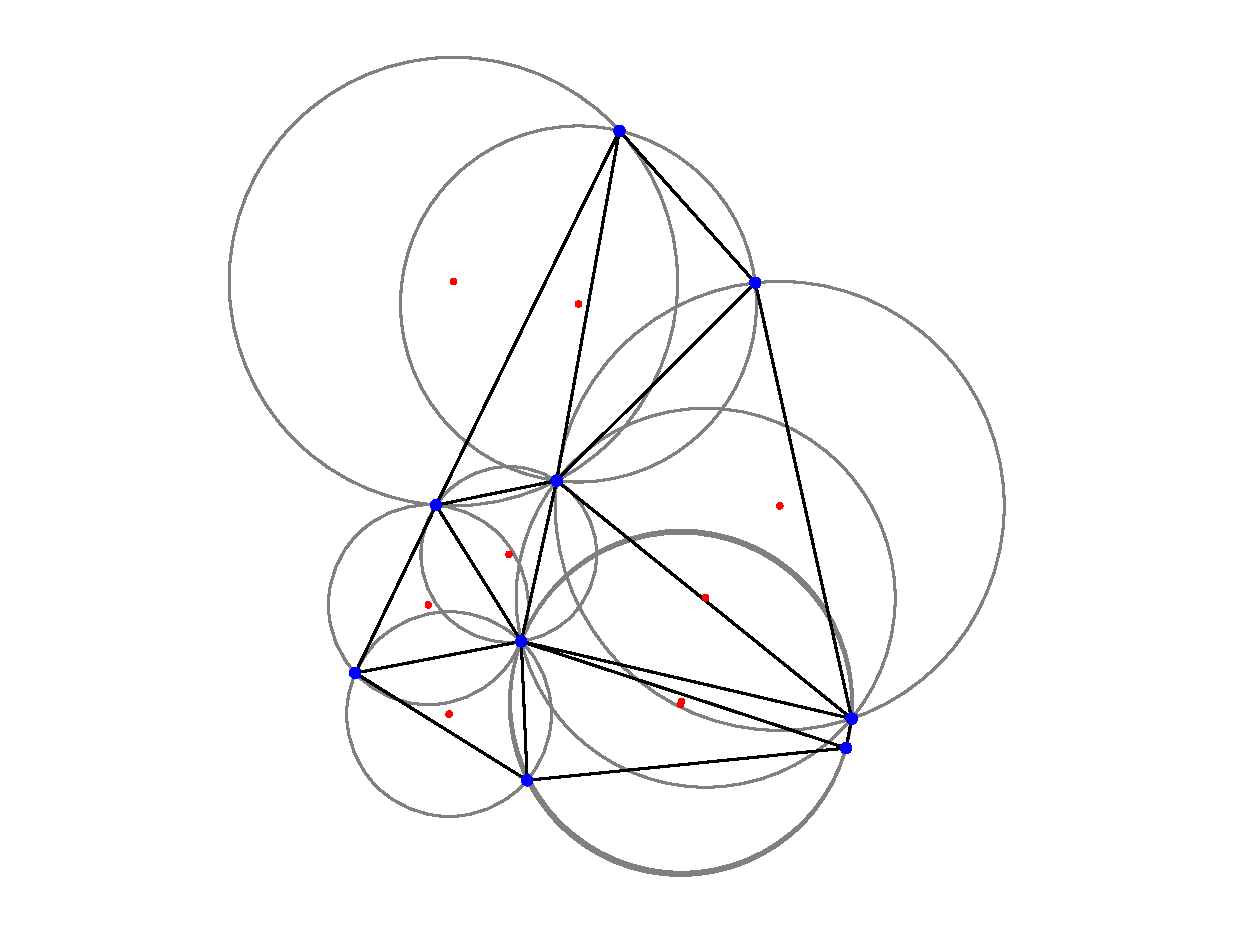
\includegraphics[scale=0.5]{fig/Delaunay-circle.eps}
\caption{The Delaunay triangulation of a set of points in the plane. The red points indicate the circumcenters. It can be seen that no vertex is within the circumcircle of some triangle.}
\label{fig:delaunay}
\end{figure}

From a practical point of view, the Delaunay triangulation offers the advantage of
producing connected graphs. However, it only comes at the cost of having a much larger edge set. In $\mathbb{R}^d, d \geq 3$, the number of triangles in the Delaunay graph is known to be $\Omega(n^{\lceil\frac{d}{2} \rceil})$. Furthermore, the worst case complexity for computing it in $d \geq 3$ is $\mathcal{O}(n^{\lceil\frac{d}{2} +1 \rceil})$ using the gift-wrapping algorithm \cite{Fortune1997}.

\begin{defn}
Let $B(x, r)$ denote the sphere or radius $r$ centered at $x$ and $\delta(p,q)$ be the distance between two points $p$ and $q$ (figure \ref{fig:erg-construct}). Let the neighborhood of two points be defined by $\Pi_{p,q} = B(\frac{p+q}{2}, \frac{\delta(p, q)}{2})$. The \termidx{Grabriel graph} (GG) of a set of vertices $V$ is such that for all edges $(p, q) \in E$  the space within $\Pi_{p,q}$ is empty. That is, $\Pi_{p,q} \cap V = \varnothing$
\end{defn}

\begin{figure}[ht]
\centering
\subbottom[GG]{%
\documentclass{standalone}
\usepackage{tikz}
\begin{document}
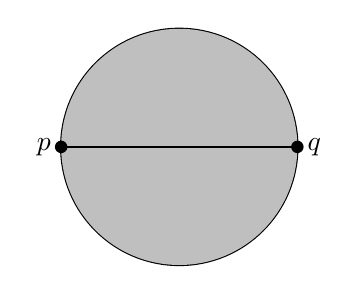
\begin{tikzpicture}[thick, scale=0.75]
\draw (0,0) circle (2cm);
\fill [gray!50] (0,0) circle (2cm);

\path (-2, 0) coordinate [label= left:$p$] (p);
\path (2,0) coordinate  [label= right:$q$] (q);
\draw (p) -- (q);
\fill [black] (p) circle (3pt);
\fill [black] (q) circle (3pt);
\end{tikzpicture}
\end{document}}
\subbottom[RNG]{
\documentclass{standalone}
\usepackage{tikz}
\begin{document}
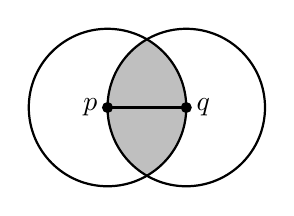
\begin{tikzpicture}[thick, scale=1.0]
\begin{scope}
\clip (-0.5,0) circle (1cm);
\clip (0.5,0) circle (1cm);
\fill[color=gray!50] (-1,1) rectangle (1,-1);
\end{scope}

\draw (-0.5,0) circle (1cm);
\draw (0.5,0) circle (1cm);
    
\path (-0.5, 0) coordinate [label= left:$p$] (p);
\path (0.5,0) coordinate  [label= right:$q$] (q);
\draw (p) -- (q);
    
\fill [black] (p) circle (2pt);
\fill [black] (q) circle (2pt);
\end{tikzpicture}
\end{document}}
\caption{Empty regions of the GG and RNG. The shaded area represents the empty region.}
\label{fig:erg-construct}
\end{figure}

The Gabriel graph was introduced in \cite{Gabriel1969} for the analysis of geographic data. In the worst case, the GG of a set of points yields $\Omega(n^2)$ edges \cite{Toussaint1992}. The expected number of edges of the GG was also studied in \cite{Devroye1988} and shown to be on the order of $2^{d-1}n$ for most probability densities. In $d$ dimensional Euclidean space, the trivial brute-force algorithm in $\mathcal{O}(dn^3)$ time complexity is the only one known to date \cite{Toussaint2012}.

\begin{defn}
The intersection of the two balls centered at $p$ and $q$ and of radius $\delta(p,q)$ respectively is called a \textit{lune} (figure \ref{fig:erg-construct}); $\Lambda_{p,q} = B(p, \delta(p,q)) \cap B(q, \delta(p,q))$. The \termidx{Relative Neighborhood Graph} (RNG) is the graph for which the set of edges $E$ is such that $(p,q) \in E 	\text{ if and only if } \Lambda_{p,q} \cap V = \varnothing$ 
\end{defn}

The Relative Neighborhood graph was introduced in \cite{Toussaint1980} and exploited for its ability to capture perceptual regularities. It was also show that in the Euclidean plane, the minimum spanning tree (MST) is a subgraph of the RNG which in turns is contained in the DT. In $\mathbb{R}^d, d > 3$, the maximum number of edges in the RNG is $\Omega(n^2)$ \cite{Toussaint1992} and the brute-force algorithm for computing it is $\mathcal{O}(n^3)$ \cite{Toussaint1980}.

\begin{defn}
The Euclidean Minimum Spanning Tree (EMST) is the minimum tree that connects every vertices with minimum weights sum. The EMST is a subgraph of the Delaunay triangulation.
\end{defn}

The fastest algorithm for computing the EMST was recently obtained by \cite{March2010} and appears to be approximately $\mathcal{O}(n \log n)$ even in $\mathbb{R}^d$.
 
 \begin{figure}
  \centering
    \subbottom[Delaunay triangulation]{%
    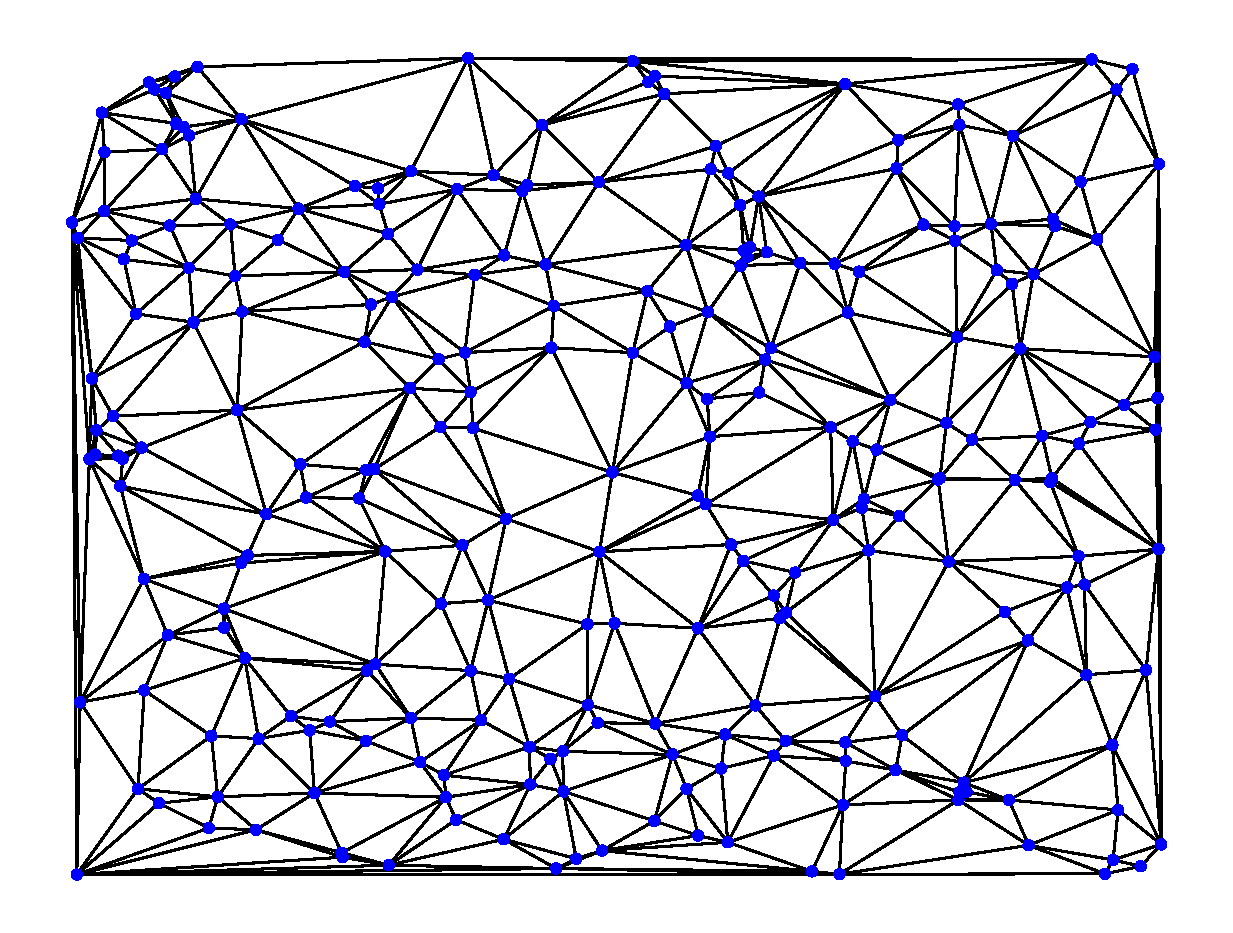
\includegraphics[width=0.45\linewidth]{fig/Delaunay-graph.eps}}
    \subbottom[Gabriel Graph]{%
    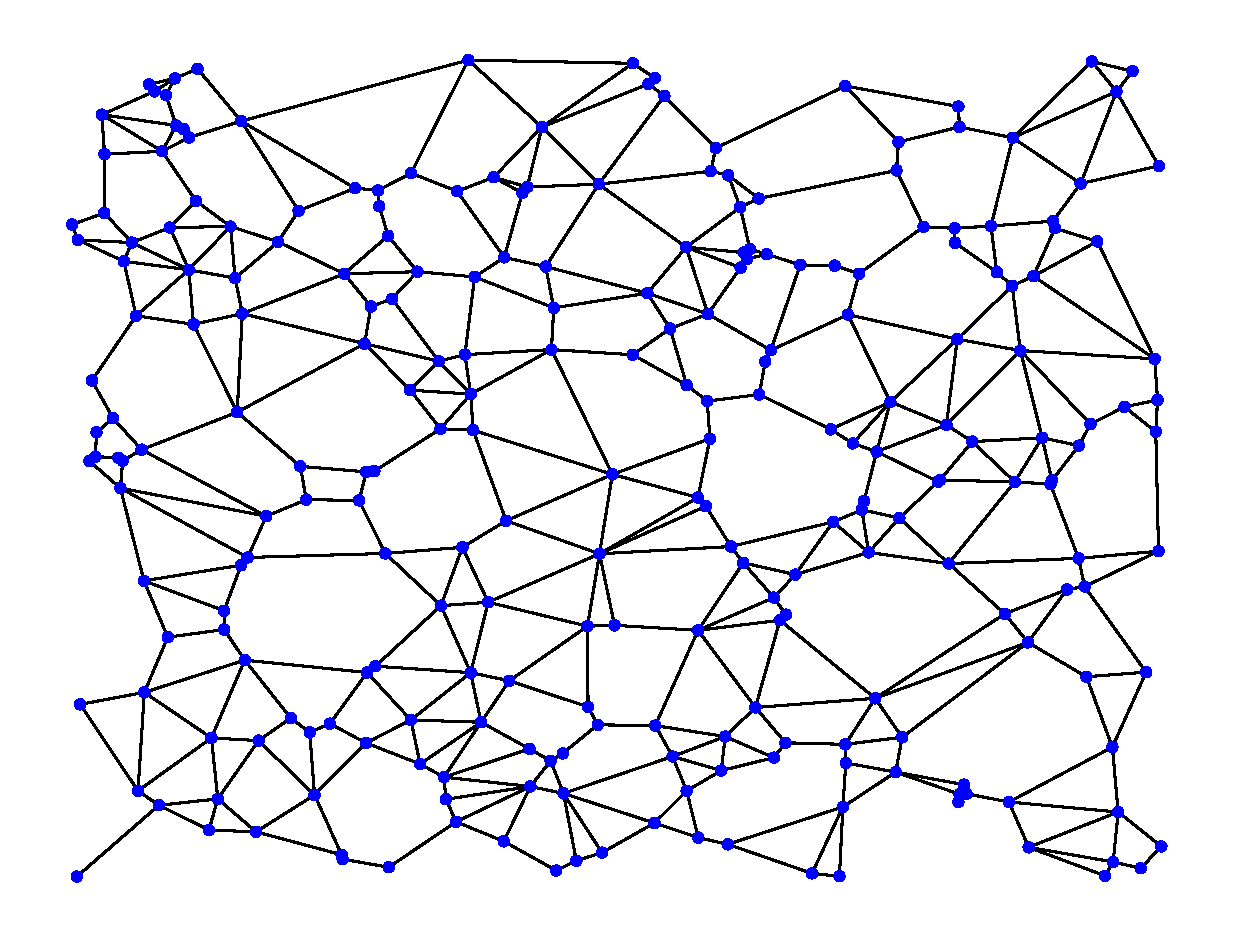
\includegraphics[width=0.45\linewidth]{fig/Gabriel-graph.eps}}
    \subbottom[RNG]{%
    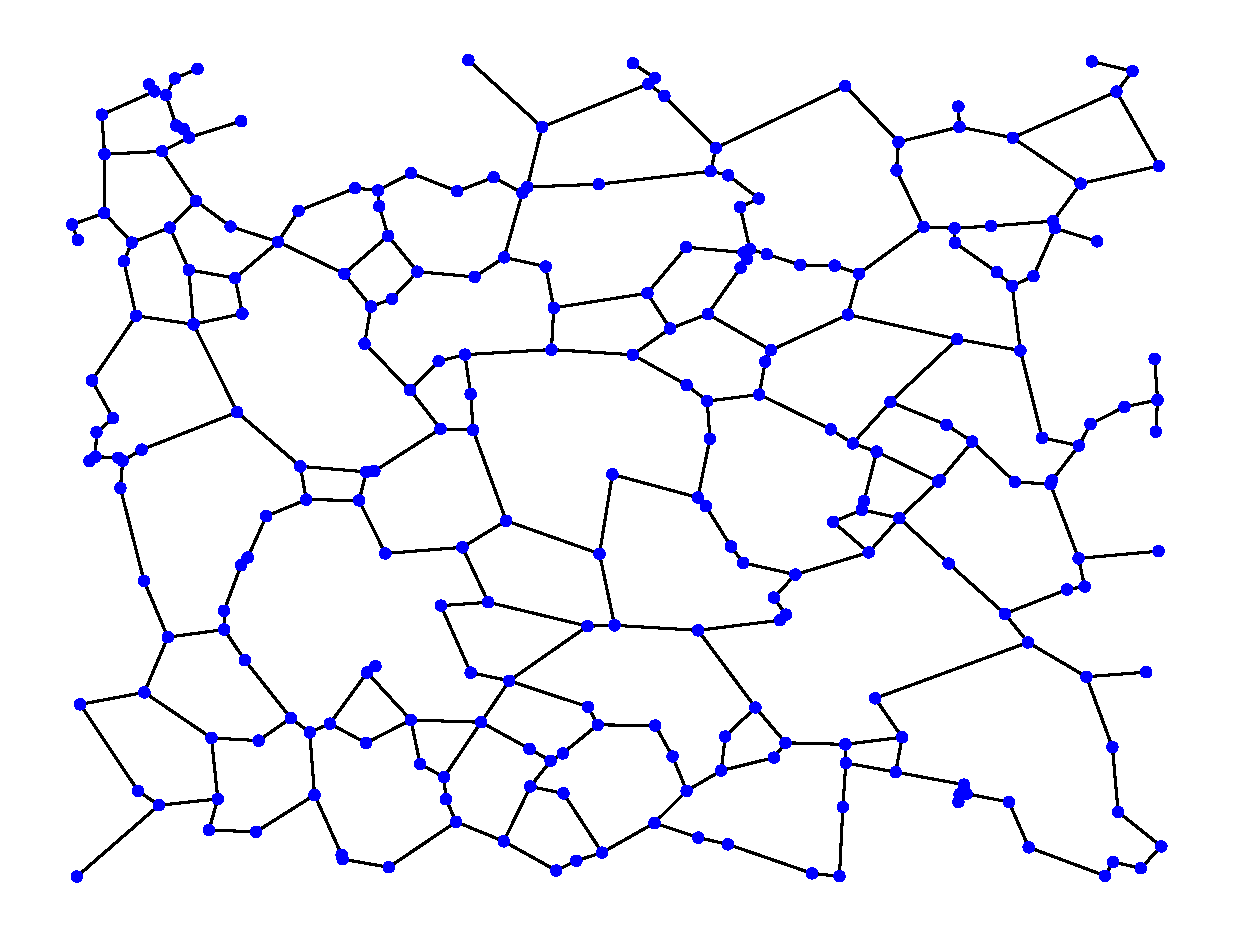
\includegraphics[width=0.45\linewidth]{fig/RNG-graph.eps}}
    \subbottom[EMST]{%
    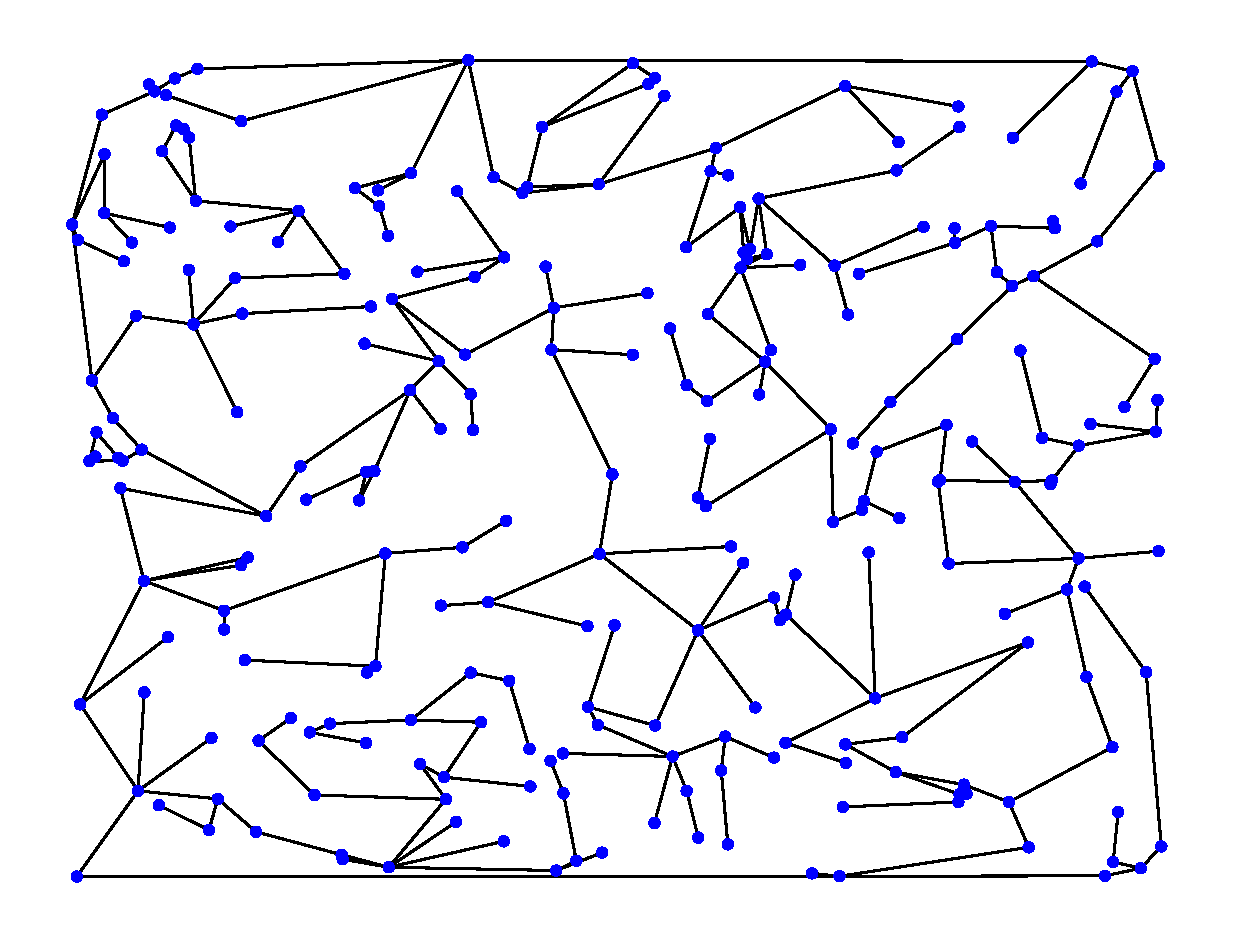
\includegraphics[width=0.45\linewidth]{fig/EMST-graph.eps}}    
    \caption{Empty region graphs, ordered according to $EMST(V) \subseteq RNG(V) \subseteq GG(V) \subseteq DT(V)$. A set of 250 points were drawn uniformly at random in $\mathbb{R}^2$}
\end{figure}

\subsection{Nearest Neighbor Graphs}

While the empty region graphs presented in the last section could be geometrically appealing, their density (exponential for the GG) is problematic. Furthermore, the computational cost for obtaining them is prohibitively expensive for the general large scale problems envisioned in this work. The class of nearest neighbor graphs tends to be a good replacement against these issues and has been prominently used in spectral clustering \cite{Luxburg2007}.

\begin{defn}
The \termidx{Nearest Neighbor Graph} (NNG) is a directed graph connecting vertex $p$ to $q$ if $q$ is the nearest neighbor of $p$.
\end{defn}

The nearest neighbor relation is not symmetric and thus forgo a definition of NNG as an undirected graph. When admitting $k$ nearest neighbors, the concept can be generalized to the K-NNG \cite{Miller1997} and the NNG appears to be only a special case where $k=1$.

\begin{defn}
The \termidx{Symmetric K-Nearest Neighbor Graph} (K-NNG) is graph for which an edge connects vertex $p$ to $q$ only if $q$ is among the $k$ nearest neighbors of $p$. Let $N_k(p)$ denote the set of $k$ points closest to $p$, the edge set is defined as
\begin{equation}
E = \{ (p, q) : p \in N_k(q) \textbf{ or } q \in N_k(p) \}
\end{equation}
\end{defn}

\begin{defn}
The \termidx{Mutual K-Nearest Neighbor Graph} (K-NNG) is graph for which an edge connects vertex $p$ and $q$ only if $q$ is among the $k$ nearest neighbors of $p$ and similarly for $q$ in the other direction. That is, 
\begin{equation}
E = \{ (p, q) : p \in N_k(q) \textbf{ and } q \in N_k(p) \}
\end{equation}
\end{defn}

\begin{defn}
The \termidx{$\epsilon$-Graph} is the graph connecting vertex $p$ and $q$ only if $q$ is within a ball of radius $\epsilon$ centered at $p$. That is, 
\begin{equation}
E = \{ (p, q) : \delta(p, q) < \epsilon \}
\end{equation}
\end{defn}

 \begin{figure}[ht]
  \centering   
    \subbottom[Input points]{%
    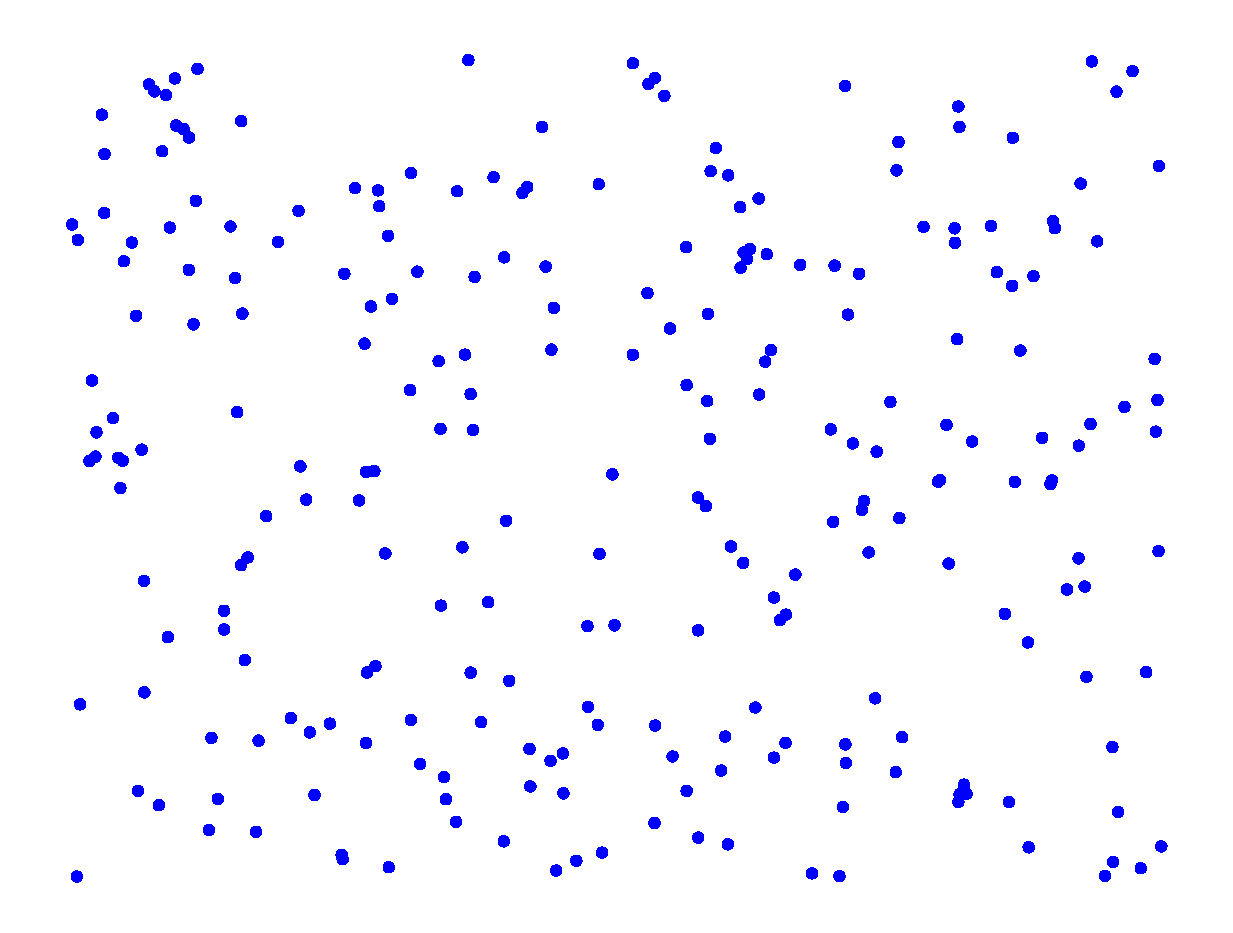
\includegraphics[width=0.45\linewidth]{fig/Points-graph.eps}}
    \subbottom[Symmetric Graph]{%
    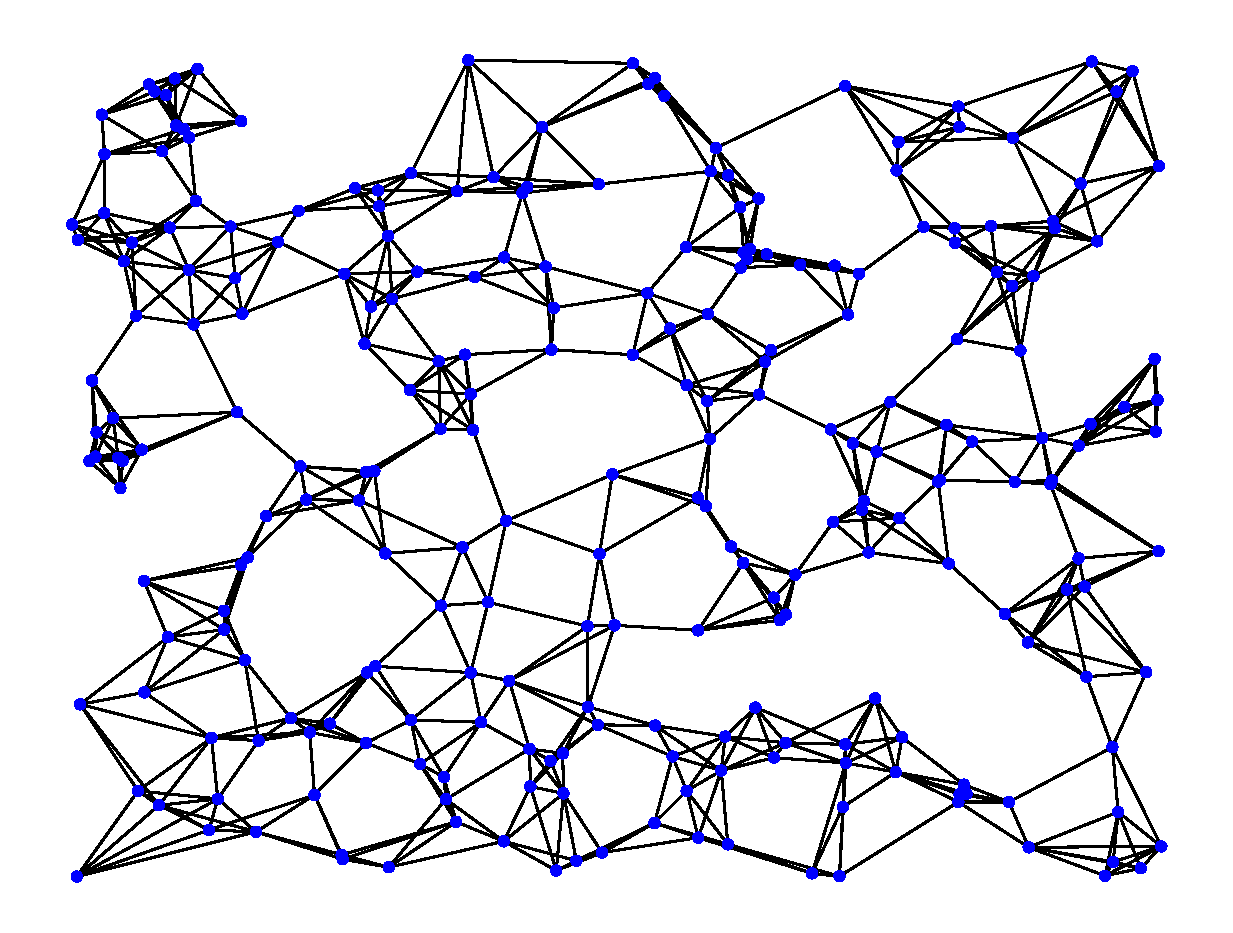
\includegraphics[width=0.45\linewidth]{fig/Symmetric-graph.eps}}
    \subbottom[Mutual]{%
    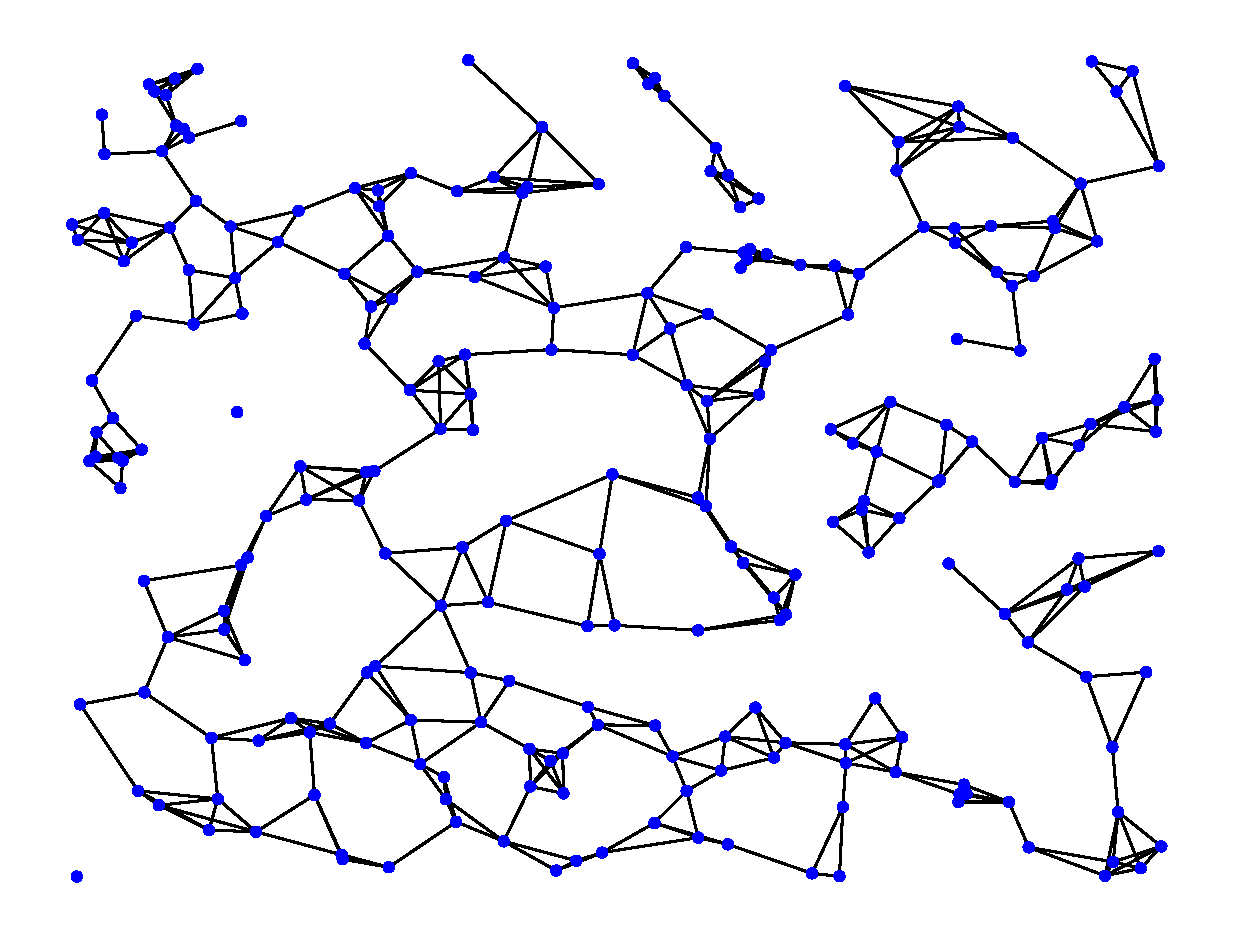
\includegraphics[width=0.45\linewidth]{fig/Mutual-graph.eps}}
    \subbottom[Epsilon]{%
    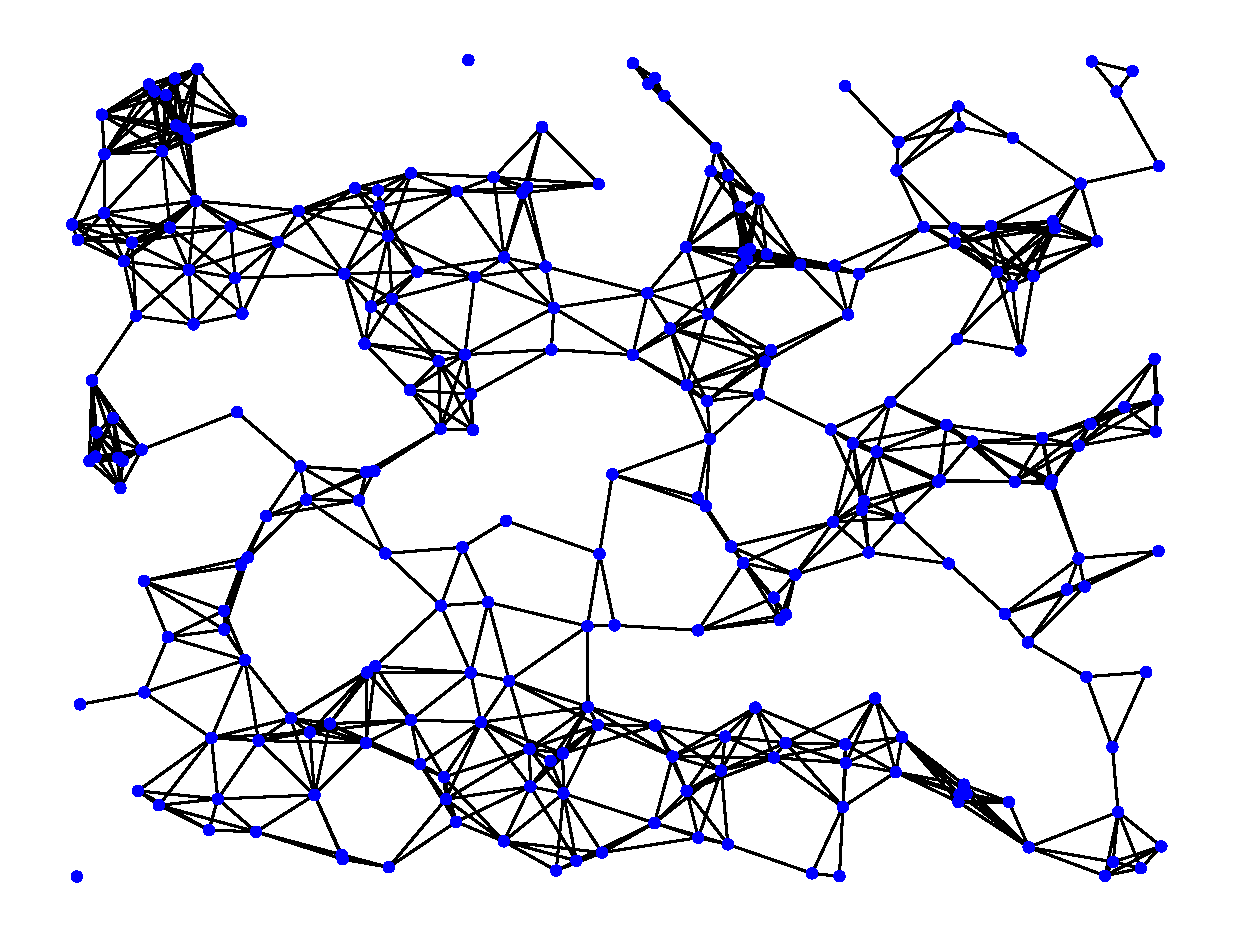
\includegraphics[width=0.45\linewidth]{fig/Epsilon-graph.eps}}   
  \caption{K-NN Graphs. The number of nearest neighbors was set to $k=5$ for the first two examples while $\epsilon$ was set to $0.01$ for the last.}
  \label{fig:knn-graphs}
\end{figure}

The choice of an appropriate radius for the $\epsilon$-graph tends to be difficult to estimate in practice. Furthermore, if the sampled data exhibit variations of density, a fixed value for $\epsilon$ will do poorly, potentially resulting in a disconnected graph. The mutual graph is usually sparser and can better function over constant densities. It however also leads more easily to  disconnected graphs as shown in figure \ref{fig:knn-graphs}. Finally, the symmetric graph better handles data at different scales but produces more edges.  

K-NN graphs can be implemented effectively using a KD-Tree \cite{Friedman1977}
structure in low dimensions but quickly suffers from the curse of dimensionality.
When allowing for approximate neighbors, very efficient algorithms have recently
been proposed to solve this problem based on the concept of \textit{locality-sensitive
hashing} \cite{Andoni2008}. As opposed to the KD-Tree approach, they perform
efficiently in high dimensional spaces. 

\section{Graph Clustering}
It has been shown in chapter \ref{chap:dynamics} how the spectral properties or the graph Laplacian can reveal the cluster structures. In general, computing the eigenvectors of dense matrices is $\mathbb{O}(n^3)$, making the $Ncut$ difficult to apply over large state spaces. The community detection algorithm of \cite{Newman2006}, the archetypical spectral clustering of \cite{Ng2001}, or the PCCA+ algorithm of \cite{Deuflhard2005} used in \cite{Mathew2012} for options discovery all exhibit the same running time.

The random walk perspective of graph partitioning is taken in the \textsc{Walktrap} algorithm of \cite{Pons2005} to reduce the time complexity which usually comes with the explicit computation of the eigenvectors. The intuition underlying this algorithm is that of a random walker visiting the graph and spending more time -- getting \textit{trapped} -- into densely connected regions and on rare occasions, jump to a different set of vertices.

This probabilistic interpretation of graph partitioning had already been exploited horoughly in the litterature on NDMC systems (section \ref{sec:ndmc}) and highlighted in \cite{Shi2001}, a corner stone for spectral clustering techniques in machine learning. The contribution of \textsc{Walktrap} might have been to show how to properly define a probabilistic distance measure between vertices and how to extract clusters from it using a fast agglomerative method.

Given the random walk transition matrix $\mathbf{P}$, the distance
measure between two vertices is defined as 
\begin{equation}
r_{ij} = \sqrt{\sum_{k=1}^n \frac{P_{ik}^t - P_{jk}^t}{d_k}} = \| D^{-1/2}
[\mathbf{P}^t]_i - D^{-1/2} [\mathbf{P}^t]_j \|_2
\label{eq:diffusion-distance}
\end{equation}

where $\| \cdot \|_2$ is the Euclidean norm and $[\mathbf{P}]^t_i$ is the
ith row of matrix $\mathbf{P}$. It appears that the same measure was
presented under the name of \textit{diffusion distance} in the same year
by \cite{Nadler2005}. Both papers also relates it to the spectrum of $\mathbf{P}$ by
showing that it amounts to explicitly computing the embedding and taking the Euclidean
distance in that space (what \cite{Nadler2005} calls the \textit{diffusion space}).
 
Intuitively, the diffusion distance measures the $L^2$ distance between two probability
distributions. The vector $[P^t]_i$ contains the probabilities of starting from vertex $i$
and reaching any other vertex $j$ in $t$ steps, taking into account all possible paths 
between them. For two vertices within a community, their probability vector are
expected to be very close as they are both likely to reach the other vertices using the
same paths. However, two vertices in different communities \textit{see} very different
sets of vertices under $t$ steps and their distance thus must be larger.\cite{Nadler2005} refers to this notion of distance as the \textit{dynamical proximity} since it depends on the dynamics of the random walk over the graph. Varying the number of steps $t$ also has for effect to expose its dynamics at different scales. In dense graphs, fewer steps are required to cover a larger portion of the graph. On the other hand, in sparser graphs larger values for $t$ would not impact as much the locality of the vertices being visited. 

The distance measure defined in equation \ref{eq:diffusion-distance} yet remains to be incorporated into a clustering scheme. Ward's agglomerative method \cite{Ward1963} is used in \textsc{Walktrap} to obtain sets of vertices which are as similar as possible with respect to this measure. Initially, the algorithm starts with $|V|$ singleton partitions.  At each iteration of the algorithm, communities are merged in a pairwise manner and the distances for the new partition is updated. The notion of distance between communities is a straightforward extension of equation \ref{eq:diffusion-distance} and expresses the probability of going from a given community $C$ to any vertex $j$ in $t$ steps.  \label{sec:walktrap}
\begin{align}
P^t_{Cj} &= \frac{1}{|C|} \sum_{i \in C} P^t_{ij} \\
r_{C_1, C_2} &= \| D^{-1/2} P_{C_1 \bullet}^t - D^{-1/2} P_{C_2 \bullet}^t\|
\end{align}

The vectors $P^t_{C\bullet}$ are thus probability distributions over the graph expressing the probabilities of choosing uniformly a vertex from $C$ and reaching some other vertex $j$ under $t$ steps. What makes Ward's algorithm efficient in this setting is that the distances after merging can be updated efficiently. Each distance computation require $\mathcal{O}(n)$ and an upper bound on this number is obtained as a function of the height of the dendogram. The number of distance computations is $\mathcal{O}(mn(H + t))$ \cite{Pons2005} (theorem 7). For sparse graphs where the number of edges $m = |V|$ and the height of the dendogram is $\mathcal{O}(\log n)$, the worst case complexity then becomes $\mathcal{O}(n^2 \log n)$. In the general case, the complexity is otherwise $\mathcal{O}(mn^2)$. 

\section{Algorithm}
\begin{algorithm}
\DontPrintSemicolon
\KwData{An environment from which to collect experience, terminal subgoal reward $R_{subgoal}$, number of random walk steps $t$, number of nearest neighbors $k$}
\KwResult{A set of options}
\SetKwData{Dataset}{dataset}
\SetKwData{Index}{index}
\SetKwData{Edges}{edges}
\SetKwData{Vertices}{vertices}
\SetKwFunction{Walktrap}{Walktrap}
\SetKwData{g}{g}
\SetKwFunction{Graph}{Graph}
\SetKwData{Communities}{communities}
\SetKwFunction{Option}{Option}
\SetKwData{Options}{options}
\SetKwData{Subgoals}{subgoals}
\SetKwFunction{Boundary}{$\partial$}
\SetKwFunction{LearnMDP}{LearnSubgoalMDP}
\;

\textbf{1. Acquire experience} \;
\Dataset $\leftarrow$ collect samples of experience $\{(x_t, a_t, x_{t+1}, r_{t})\}$ through some fixed policy. A random walk process can be used if the optimal policy is not known. \;
\Dataset $\leftarrow$ optionally subsample the dataset uniformly at random if too large\;
\Index $\leftarrow$ build an approximate nearest neighbor index over the sampled states\;
\;
\textbf{2. Build the symmetric K-NN graph}\;
\Vertices $\leftarrow $ set of sampled $x_t$ in \Dataset \;
\Edges $\leftarrow \varnothing$\;
\ForEach{state $x$ in dataset} {
knn $\leftarrow$ query the $k$ nearest neighbors of $x$\;
  \ForEach{nearest neighbor $nn$ in knn} {
    \If{$nn$ is in knn} {
    \Edges $\leftarrow$ \Edges $\cup \; (x, nn)$
    }
  }
}
\;
\textbf{3. Discover and learn options} \;
\Communities $\leftarrow$ \Walktrap{\Graph{\Vertices, \Edges}, t} \;
\Options $\leftarrow \varnothing$ \;
\ForEach{community c in \Communities} {
  $\mathcal{I} \leftarrow c$\;
  \Subgoals $\leftarrow \partial(c)$\;
  $\beta \leftarrow \indicator_{\Subgoals}$ \;
   $\g \leftarrow \indicator_{\Subgoals}\cdot R_{subgoal}$\;
   $\pi \leftarrow$ \LearnMDP{\g} \;
   \Options $\leftarrow$ \Options $\; \cup \;$ \Option{$\mathcal{I}$, $\beta$, $\pi$} \;
}
\Return \Options
\caption{\textsc{Bottleneck-Options} construction algorithm}
\label{alg:knnoptions}
\end{algorithm}

A fast method for discovering and learning subgoal options is presented in algorithm \ref{alg:knnoptions}. For each option, a terminal subgoal value (pseudo-reward) $g$ is overlaid to the underlying reward function of the global MDP. The type of features or optimal control algorithm is left unspecified. In the experiments presented in the next chapter, Fourier features and SARSA were used. The Least-Square Policy Iteration (LSPI) \cite{Lagoudakis2003} algorithm could equally do well while making efficient use of the batch data collected in the first step. In order to make the algorithm capable of handling large state spaces, the \textsc{Walktrap} algorithm is used to discover dynamically stable regions of the state space from the random walk process. 

The symmetric K-NN proximity graph construct was retained for its computational efficiency, better adaptation across different scales and sparsity. In the spectral clustering literature the problem of obtaining a similarity graph is sometimes neglected by simply assuming a complete graph with $n^2$ edges. Such a dense representation however quickly leads to poor computational performance. K-Nearest Neighbor graphs are also used for spectral clustering and their empirical properties are  discussed in \cite{Luxburg2007}. The family of empty regions graphs consisting of the beta-skeleton graph, GG and RNG was also investigated in \cite{Correa2012}. The use of EMST graphs was ruled out in this algorithm because of its extreme sparsity. It is worth nothing however that \cite{Carreira2004} experimented with ensemble of \textit{perturbed} EMST. The resulting denser combined graph was reported to perform well for clustering.

In practice, the choice of $k$ will dramatically impact the clustering. It is often desirable to simply settle on a value which leads to a connected graph. Little is known in the spectral clustering literature about the effect of this parameter and even less about the general problem of choosing an suitable proximity graph construct. \cite{Maier2008} provides some theoretical results about the convergence of graph clustering as a function of $k$ but fail to provide practical guidelines. 

\subsection{Initiation and Termination in Continuous Space}
\label{sec:knnoptions}
When applying algorithm \ref{alg:knnoptions} in continuous state spaces, the definition of the initiation and termination components needs to be generalized over regions rather than discrete states. Having already constructed a nearest neighbor index for  the proximity graph, an efficient solution is to use it in the definition of the termination function. 

\begin{equation}
\beta(x) = 
\begin{cases}
1 & \text{if } N_1(x) \in C_x\\
0 & \text{otherwise}
\end{cases}
\end{equation}

where $N_1(x)$ is the first NN of $x$ and $C_x$ stands for the community to which $x$ was found to belong to. For better robustness against noise, $k$ nearest neighbors can be queried for their majority vote.

Membership to the initiation set can be determined by negating the effect $\beta$. Let $C$ be the community associated with some initiation set of an option, a membership query consists in
\begin{equation}
N_1(x) \in C \Rightarrow x \in C  \\
\end{equation}

Once again, majority voting can be used to reduce the effect of noise. 


%%%%%%%%%%%%%%%%%%%%%%%%%%%%%%%%%%%%%%%%%%%%%%%%%%%%%
% Experiments
%%%%%%%%%%%%%%%%%%%%%%%%%%%%%%%%%%%%%%%%%%%%%%%%%%%%%
\chapter{Empirical Evaluation}
\label{chap:illustration}
The Pinball domain \cite{Konidaris2009} was chosen to better understand the practical implications of the options construction algorithm presented in the last chapter. This environment consists in arbitrarily shaped obstacles laid out on the plane between and among which an agent must learn to navigate a ball to the target (figure \ref{fig:pinball}). The agent has access to four primitive discrete actions which increase or decrease the velocity of the ball in the $x$ and $y$ directions as well as a fifth \textit{null} action. Collisions with the obstacles are elastic and a drag coefficient of 0.995 effectively stops ball movements after a finite number of steps when the null action is chosen repeatedly. Each thrust action incurs a penaly of -5 while taking no action costs -1. The episode terminates with +10000 reward when the agent reaches  the target. A four-dimensional continuous observation vector $[ x, y, \dot{x}, \dot{y}]$ is available to the agent at every time step and can quickly exhibit sharp discontinuities under poor controllers. While the pinball environment as presented originally in \cite{Konidaris2009} is purely deterministic, normal noise with standard deviation $\sigma = 0.03$ was added exactly as in \cite{Tamar2013}. 

\begin{figure}
\centering
\subbottom[Pinball]{\includegraphics[width=0.32\textwidth]{fig/pinball.pdf}\label{fig:pinball}}%
\subbottom[Graph construction and pruning]{\includegraphics[width=0.325\textwidth]{fig/pinball-graph-pruned.png}\label{fig:pinball-graph-pruning}}%
\subbottom[Graph clustering]{\includegraphics[width=0.32\textwidth]{fig/pinball-clustering.pdf}}
\caption{Pinball domain for reinforcement learning}
\end{figure}

For easier comparison with the results presented in \cite{Konidaris2009}, the obstacles layout named \texttt{pinball\_simple\_single.cfg} from the open source implementation \footnote{\url{http://www-all.cs.umass.edu/~gdk/pinball/}} of the author was used. It has been chosen to implement \footnote{\url{https://github.com/pierrelux/pypinballl}} Pinball in Python rather than using the Java package already made available. One reason for this was to simplify the integration with the Python-RL \footnote{\url{https://github.com/amarack/python-rl}} project from which some components had been used. Great care has however been taken in ensuring that the two implementations behave exactly the same. 

\section{Graph Construction}

Instead of collecting samples from a random walk process, a Sarsa($\lambda$) agent was trained with $\alpha = 0.001, \gamma = 0.9, \lambda = 0.9, \epsilon 0.01$ and 50 trajectories were collected from it. This choice was motivated by the practical need of keeping the number of samples as low as possible while favoring the most relevant one. The set or trajectories was then merged into one dataset consisting in 48060 sampled states. While this number represents the order of magnitude for which the algorithm was intented, the dataset was uniformly subsampled down to 5000 data points for easier empirical exploration. 

The \texttt{FLANN} library of \cite{Muja2009} was then used to build an approximate nearest neighbors index for the construction of the symmetric KNN graph represented with the data structures of the \texttt{igraph} library of \cite{Csardi2006}. The choice of the number of nearest neighbors $K$ was based on an empirical evaluation and the objective of keeping it as small as possible while minimizing the number of communities found by \textsc{Walktrap} and maximizing the so-called \textit{modularity}. A given graph partitioning among $c$ clusters or \textit{modules} has a high value of modularity when the density of connections within a module is high compared to the inter-module ones. The definition of this measure was given in \cite{Newman2006} as
\begin{align}
Q &= \sum_{i}^c \left( e_{ii} - a_i^2 \right) \\
e_{ii} &= \sum_j 	\frac{A_{ij}}{2m} \delta(c_i, c_j) \\
a_i &= \sum_j e_{ij}
\end{align}

The $e_{ii}$ term here above is the fraction of edges within community $i$ while $a_i$ is of those edges with at least one vertex in $i$. \textsc{Walktrap} does not directly optimizes on modularity but rather uses the diffusion-like distance as presented in section \ref{sec:walktrap}.
The vertex dendogram produced by Ward's algorithm is however chosen to be cut at its maximum of modularity. 

\begin{figure}
\centering
\subbottom[From top to bottom: influence of the number of nearest neighbors on the number of edges, number of communities and modularity. Averaged over 10 graphs for each $K$]{\includegraphics[width=0.49\textwidth]{fig/knn-influence.pdf}\label{fig:knn-vs-clusters}}\hspace{2mm}%
\subbottom[From top to bottom: influence of the number of random walk steps on the number of communities found and associated modularity.]{\includegraphics[width=0.49\textwidth]{fig/steps-influence.pdf}\label{fig:steps-vs-clusters}}
\label{fig:pinball-graph}
\caption{Effect of $K$ and $t$ during graph construction and clustering}
\end{figure}

As $K$ increases, the graph becomes denser and drives the communities to be more compact and less numerous. \textsc{Walktrap} being $\mathcal{O}(mn^2)$, higher values of $K$ also have a direct impact on the running time as the number of edges $m$ gets larger. The presence of error bars in figure \ref{fig:knn-vs-clusters} is due to the approximate nearest neighbour graph construction which results in probabilistic edge assignment. As $K$ gets larger, the graph gets denser and that the clustering seems to become more stable. Intuitively, adding more edges in an already dense graph should have less of an impact on the inter-community probabilities than in a sparse one. A perturbation analysis could shed some light on this phenomenon. Based on the curves shown in figure \ref{fig:knn-graphs}, $K=25$ was retained for this experiment as it yielded good clustering stability and an edge set $|E| = 90348$ of tractable size. 

The number of random walk steps in \textsc{Walktrap} affects the scale at which the dynamical proximity is measured. As discussed in section \ref{sec:walktrap}, the graph density should be considered in this choice. For large values of $K$, the resulting denser graph will blur away faster the difference between any pair of vertices under longer random walks. Figure \ref{fig:steps-vs-clusters} shows this phenomenon starting from $t=8$ where the number of communities sharply decreases from 26 to 16 as the vertices get dynamically more similar. A smaller number of time steps $t=4$ was deemed appropriate for this experiment, providing big enough communities, a modularity of 0.7852 and fast computation.

A post-processing step was added in this experiment in order to prune infeasible edges and improve the graph representation. In the Pinball domain, the observation space calls for a graph representation where edges are set between four-dimensional Euclidean points of the form $[x, y, \dot{x}, \dot{y}]$. While it can difficult to establish the feasibility of a transition between any two such points, it is clear that no edge should cross the obstacles in the x-y plane. A line intersection test is thus performed over the symmetric graph to remove any such edge (figure \ref{fig:pinball-graph-pruning}). The options construction algorithm can be dispensed with this step in the absence such domain specific knowledge. The experience gathered during this experiment has however shown that it can greatly improve the clustering quality.

\section{Learning}

\begin{figure}
\centering
\subbottom[The flat policy take more episodes to achieve the same number of steps as the one over options]{\includegraphics[width=0.49\textwidth]{fig/sarsa-intra.eps}}\hspace{2mm}%
\subbottom[Bottleneck options produce uncontrollable oscillatory behavior at the boundary]{\includegraphics[width=0.49\textwidth]{fig/pinball-bottleneck.eps}\label{fig:pinball-bottleneck}}
\caption{Learning with options}
\end{figure}

The bottleneck options algorithm \ref{alg:knnoptions} was applied over the clustering for the definition of the initiation, policy and termination components of the options. The bottleneck construction seek option policies which can bring the agent at the boundary of their respective cluster from any state within the initiation set. It has been found however that the \textit{vanilla} bottleneck concept appears to be flawed when it comes to the continuous case. Indeed, the canonical reinforcement learning domain for motivating the bottleneck concept has been mainly concerned with the \textit{doors and rooms} domains in discrete state space. In an environment such as the four rooms domain \cite{Sutton1999}, bottlenecks are precisely those single rectangular cells connecting two rooms in the x-y plane. 

The situation becomes much more complex for the type of community structures found in Pinball. The problem is twofold: the number of adjacent communities is larger and the bottleneck regions are wider. The difficulty stems mostly from the fact that bottlenecks are now identified in a four-dimensional space rather than only across xy coordinates. In the four-rooms domain, learning a policy which bring the agent to any of its two doors arbitrarily at random would not impact the rate of convergence as much. Generally, the agent should however be constrained to an optimal stochastic choice about which of the bottleneck states on the boundary should be reached in order to obtain maximal payoff. Furthermore, as the number of adjacent communities gets larger, the number of possible outcomes arising from a transition to any of them might increase and become also more difficult to evaluate. This intuition as verified empirically by training the bottleneck options using the Sarsa($\lambda = 0.9$) algorithm with learning rate $\alpha = 0.001$, discount factor $\gamma = 0.9$ and an epsilon-greedy exploration strategy with $\epsilon = 0.01$. A policy over such options was then obtained using the Intra-Option learning with $\alpha = 0.001, \gamma = 0.9, \epsilon = 0.01$. A linear fourth-order Fourier approximation of the action-value function for every, flat or options-based agent. Figure \ref{fig:pinball-bottleneck} compares the number of steps taken per episode with that of a flat Sarsa($\lambda$) learning agent. The latter shows steady convergence to some successful policy which can take the ball from its initial position to the goal. No learning however seems possible under the naive bottleneck construction and intra-option learning is very unstable. 

\section{Navigation Options}

The need to impose a stochastic choice as to which bottlenecks to reach on the boundary lead to slightly different kind of options referred to as \textit{navigation options}. The chosen designation highlights the fact that such an option specifies a policy to \textit{navigate} between a fixed pair of adjacent communities.

\begin{algorithm}
\DontPrintSemicolon
\KwData{An environment from which to collect experience, terminal subgoal reward $R_{subgoal}$, number of random walk steps $t$, number of nearest neighbors $k$}
\KwResult{A set of options}
\SetKwData{Dataset}{dataset}
\SetKwData{Index}{index}
\SetKwData{Edges}{edges}
\SetKwData{Vertices}{vertices}
\SetKwFunction{Walktrap}{Walktrap}
\SetKwData{g}{g}
\SetKwFunction{Graph}{Graph}
\SetKwData{Communities}{communities}
\SetKwFunction{Option}{Option}
\SetKwData{Options}{options}
\SetKwData{Subgoals}{subgoals}
\SetKwFunction{Boundary}{$\partial$}
\SetKwFunction{LearnMDP}{LearnSubgoalMDP}
\SetKwFunction{Mode}{Mode}
\SetKwData{Adjacencies}{adjacencies}
\SetKwData{ModeLabel}{label}
\SetKwData{ModeFreq}{frequency}
\SetKwData{KNN}{knn}
\SetKwData{Membership}{membership}
\SetKwData{Label}{label}
\SetKwData{AdjLabel}{adjLabel}
\;

\textbf{1. Acquire experience} \;
\textbf{2. Build the symmetric K-NN graph}\;
\textbf{3. Discover and learn options} \;
\textbf{3.1 Establish relevant adjacent communities}\;
\Communities $\leftarrow$ \Walktrap{\Graph{\Vertices, \Edges}, t} \;
\Adjacencies $\leftarrow \underbrace{[ \varnothing, \dots, \varnothing]}_{|\Communities|}$\;
\ForEach{community c \KwSty{in} \Communities} {
  \ForEach{node n \KwSty{in} c} {
     \KNN $\leftarrow$ query the $k$ nearest neighbors of $n$\;
     \ModeLabel, \ModeFreq $\leftarrow$ \Mode{\KNN} \;
     \If{\DataSty{label} $\not =$ \DataSty{membership[n]} \KwSty{and} \DataSty{frequency} $\geq \lceil \frac{k}{2} \rceil$} {
        $\Adjacencies[\Membership[n]] \leftarrow \Adjacencies[\Membership[n]] \cup \Label$\;
      }
    }
}
\textbf{3.2 Learn options}\;
\Options $\leftarrow \varnothing$ \;
\ForEach{$\langle \Label , \AdjLabel \rangle$ \KwSty{in} \Adjacencies} {
  $\mathcal{I} \leftarrow \Communities[\Label]$\;
  $\Subgoals \leftarrow \Communities[\AdjLabel]$\;
  $\beta \leftarrow \indicator_{\Subgoals}$ \;
   $\g \leftarrow \indicator_{\Subgoals}\cdot R_{subgoal}$\;
   $\pi \leftarrow$ \LearnMDP{\g} \;
   \Options $\leftarrow$ \Options $\; \cup \;$ \Option{$\mathcal{I}$, $\beta$, $\pi$} \;
}

\Return \Options
\caption{\textsc{Navigation-Options} construction algorithm}
\label{alg:navoption}
\end{algorithm}

Algorithm \ref{alg:navoption} is identical that of \ref{alg:knnoptions} on the sampling and graph construction steps. It however differs in the option discovery and construction approach by defining options \textit{between} communities. The adjacent communities could be discovered simply by considering the bottleneck edges and the label of their adjacent vertices. While this approach would be valid in a perfect graph representation, the identification of relevant bottleneck states is hindered by the high edge density found to be necessary for obtaining a satisfactory clustering. Under such densities, most vertices of a community are also bottleneck states. It is thus desirable in practice to identify adjacent communities on the basis of a sparser proximity graph. Algorithm \ref{alg:navoption} for navigation options thus queries the $k$ nearest neighbors and the most frequent label appearing among them is subject to majority test before establishing the adjacency relation. This procedure both reduces the number bottleneck outliers and irrelevant adjacent communities, which in the worst case could otherwise result in $|C|^2$ many navigation options.

\begin{figure}
\centering
\includegraphics[width=0.49\textwidth]{fig/pinball-nav.pdf}
\caption{Navigation options found using algorithm \ref{alg:navoption}. Each arrow corresponds to an option policy for transitioning across the given pair of communities. Macro transitions 1 to 7, 5 to 6, 6 to 1, and 7 to 0 were then manually selected for learning.}
\label{fig:nav-options}
\end{figure}

The navigation options construction algorithm was applied over the 18 communities found by \textsc{Walktrap} at maximum modularity under $t=4$. It lead to 34 adjacency relations being established, pruning at the same time small communities consisting of only a few vertices. The learning curve in figure \ref{fig:nav-options} was obtained by averaging 10 \textsc{Intra-Option} learning agents with $\alpha = 0.1, \gamma = 0.9, \epsilon = 0.1$ and a fourth order Fourier approximation. 

While offering the powerful off-policy property, \textsc{Intra-Option} is known to diverge with function approximation. Such a difficulty was encountered during experimentation and motivated the decision to manually select a subset of four options from the 34 found automatically. Such a simplification reduced the learning complexity and made the painstaking task of finding suitable learning parameters more easy. The options set used in \ref{fig:nav-options} thus consisted of the five primitive actions of pinball augmented with these four navigation options. From the very few first episodes, it can be seen that the agent having access to options successfully learnt to reach the target under approximately 300 steps while the Sarsa agent having access to only primitive actions flattens off above 1000. 

%\begin{figure}
%\centering
%\subbottom[Intra-Option learning can diverge with function approximation]{\includegraphics[width=0.49\textwidth]{fig/intra-diverge.eps}}
%\end{figure}

%%%%%%%%%%%%%%%%%%%%%%%%%%%%%%%%%%%%%%%%%%%%%%%%%%%%%
% Conclusion
%%%%%%%%%%%%%%%%%%%%%%%%%%%%%%%%%%%%%%%%%%%%%%%%%%%%%
\chapter{Conclusion}
The bottleneck approach to options discovery can appear rebuttal because of the lack of proper theoretical foundations. This thesis attempted to motivate this family of heuristics by establishing a connection to spectral graph theory and relating it to the vast body of work on Nearly Decomposable Markov Chains (NCD) spanning across more than three decades. Furthermore, an algorithm based on these principles was proposed for discovering options in continuous state spaces. While many bottleneck-like approaches have succeeded in applying them to discrete domains, none had yet shown how to extend these ideas in a continuous domain such as Pinball. The empirical evaluation of the proposed algorithm showed its feasibility but also highlighted practical difficulties to use it as a \textit{black-box} approach.

A frequent critique brought against this class of algorithms has to do with the reward structured being apparently ignored. After having studied the properties of the graph Laplacian in section \ref{chap:dynamics}, this claim can be dismissed. It is true that algorithm proposed here constructs a graph representation which does not capture the underlying transitions probabilities of some MDP. The resulting clustering can then be understood in terms of the dynamics of a random walk process over it; a different stochastic process than the MC induced by some policy. Bottlenecks captured in this way are thus related to those of the random walk Laplacian rather than the original Laplacian of the MDP. If such a substitution does not preserve the reward structure, how can it then succeed in practice ?

A plausible reason might have to do with the kind of domains commonly chosen in HRL. In the four-rooms domains for example, doors appear as natural bottleneck states but also happen to be in structural elements in solution space. The four-rooms domain is so ubiquitous that bottlenecks are often explained in terms of doors. Such references have the unfortunate effect of misguiding practitioners into conceiving bottlenecks as merely \textit{state features}, or \textit{saliencies}, rather than as an effective \textit{coarsening} of the dynamics induced by an MDP.

The empirical results presented in this work depart from those obtained by previous authors in the fact that a bottleneck-like option construction algorithm for continuous state space was proposed and evaluated under a new HRL domain. While subject to the same oversimplification concerning the reward structure, a useful options decomposition was still obtained in the Pinball domain, but also uncovered practical obstacles. 

It seems at this point that a proper research methodology should be concerned with not only a more diverse set of domains but also consider the generation of random MDPs with varying degrees of decomposability. The approach of \cite{Archibald1995} for the generating MDPs seems to be an appropriate fit with the mixing rate being controllable as well as other structural properties of the transition matrix. 

The recurrence of the bottleneck concept in the literature should motivate the establishment of a research agenda to equip the notion with proper theoretical foundations. The theory of NCD Markov chains, and more generally that of MDPs from operations research, seems to have been overlooked in in HRL. The problem of options discovery should be first tackled using the theory of MDPs and extended to more of model-free and online setting compatible with the reinforcement learning framework. A promising research avenue might lie in some information theoretic approach similar to \cite{Deng2011} under a rate distortion perspective of the value function as initiated by \cite{Still2012}. Such results would not only benefit our understanding of temporal abstraction in RL but also provide insights to the line of work initiated by \cite{Botvinick2012} on the cognitive process involved in human subgoal discovery.


%%%%%%%%%%%%%%%%%%%%%%%%%%%%%%%%%%%%%%%%%%%%%%%%%%%%%
% Bibliography
%%%%%%%%%%%%%%%%%%%%%%%%%%%%%%%%%%%%%%%%%%%%%%%%%%%%%
%\bibliography{library}
%\bibliographystyle{plain}
\printbibliography
\end{document}